\documentclass[11pt, a4paper]{report}   	% use "amsart" instead of "article" for AMSLaTeX format

\usepackage{geometry}
\usepackage[parfill]{parskip}    		% Activate to begin paragraphs with an empty line rather than an indent
\usepackage{graphicx}				% Use pdf, png, jpg, or eps with pdflatex; use eps in DVI mode
\usepackage[english, american]{babel}
\usepackage{csquotes}
\usepackage{xr} % Fross cross-referencing between multiple tex-files
\usepackage{caption} % Removes [:] in figure captions
\usepackage{placeins}
\usepackage[utf8]{inputenc}
\usepackage{amssymb}
\usepackage{amsmath}
\usepackage{bm}
\usepackage{amsthm}
\usepackage{stmaryrd}
\usepackage{verbatim}
\usepackage{enumerate} % Pretty lists with (i),(ii)...
\usepackage{color}
\usepackage{ebproof}
\usepackage{tikz}
\usepackage[style=ieee, citestyle=numeric, backend=biber]{biblatex}
\DeclareLanguageMapping{american}{american-apa}
\addbibresource{reference.bib}

\theoremstyle{plain}
\newtheorem{theorem}{Theorem}
\newtheorem{conjecture}[theorem]{Conjecture}
\newtheorem{corollary}[theorem]{Corollary}
\newtheorem{lemma}[theorem]{Lemma}

\theoremstyle{definition}
\newtheorem{definition}[theorem]{Definition}
\newtheorem{example}[theorem]{Example}

%The following group solves the theorem-spacing problem caused by parskip
\begingroup
  \makeatletter
  \@for\theoremstyle:=definition,plain\do{%
    \expandafter\g@addto@macro\csname th@\theoremstyle\endcsname{%
      \addtolength\thm@preskip\parskip
      }%
    }
\endgroup

\newcommand{\lar}{\leftrightarrow}
\newcommand{\todo}[1]{\footnote{\textcolor{red}{TODO:} #1}}
\newcommand{\ol}[1]{\overline{\vphantom{b}#1}}

\usetikzlibrary{matrix}
\usetikzlibrary{positioning}

\def\name{Kjetil Midtgarden Golid}
\title{
{\fontsize{28}{36}Incompleteness of the Inference System BNeg}
	\author{
	\name\vspace{3cm}\\
		\includegraphics[width=74mm]{figures/uglo}\vspace{2em}\\
		Master Thesis\vspace{2em}\\
		Department of Informatics\\
		University of Bergen
	}
	\date{\today}
}

\begin{document}
	\maketitle
  \begin{abstract}
    Any propositional discourse can be represented as a propositional theory in a specific form in such a way that the theory is inconsistent if and only if the discourse is paradoxical.
Propositional theories in this form can be represented as directed graphs such that the models of the theory correspond to the kernels of the digraph.
This thesis looks at a sound, refutationally complete, non-explosive resolution system over such propositional theories.
We investigate the relation between various graph structures and clauses provable by the resolution system from the corresponding theory.
We also show that a restricted version of the resolution system is \textit{not} refutationally complete.

  \end{abstract}
	\tableofcontents
  \chapter{Introduction and Preliminaries}
  \label{chap:Introduction}
  % !TEX root= ../main.tex
\section{Paradoxes}
\label{sec:Paradoxes}
A theory in propositional logic is semantically \textit{inconsistent} if it has no model, i.e., there exists no variable assignment making all formulae in the theory true.
Consider the following example:
\begin{align}
  x \wedge \neg x
\end{align}
While a sentence like $\neg a \rightarrow b$ can be satisfied by, for instance, letting both $a$ and $b$ be true, no such assignment can be made for the statement above.
The statement is therefore inconsistent.

A paradox is usually informally defined as something along the lines of \textit{``a statement that can be neither true nor false''}.
We can immediately note one thing from this intuitive definition:
Since no paradoxes can be true, all paradoxes are, by definition, inconsistent.
It is however not the case that all inconsistent theories are paradoxes.
Just consider the inconsistent statement, $x \wedge \neg x$ again: this statement simply seems false, and not paradoxical.

A different view is that a paradox is a \textit{dialetheia}, a sentence that is \textit{both} true and false\cite{sep-dialetheism}. We will however not spend much time exploring these philosophical differences, as this is not a philosophical paper and it won't change much for our definitions.

The liar sentence is probably the most famous example of a paradox:
\begin{quote}
  ``This sentence is false.''
\end{quote}
If the statement is true, then the statement is false, but if the statement is false, then the statement is true.
It can thus neither be true nor false, since both lead to a contradiction.

Notice how the liar sentence is a statement about other statements (in this case itself).
A collection of statements where some of them may refer to themselves or other statements, is called a \textit{discourse} in \cite{synthese-pdl}, which we will follow.
In order to represent such discourses, we need a formal way of referencing other statements within statements.
In propositional logic, this can be done simply by giving statements ``names'' in the form of adding fresh variables with equivalences to their corresponding statements\todo{bad wording?}.

Consider the examples below; with normal propositional statements to the left, together with the corresponding \textit{named} statements to the right.
\begin{align}
  a               && x_1 \leftrightarrow a\\
  a \wedge \neg a && x_2 \leftrightarrow a \wedge \neg a\\
  a \vee \neg a   && x_3 \leftrightarrow a \vee \neg a
\end{align}
Labelling statements in this way obviously changes their truth value.
Even though we have one consistent, one inconsistent and one tautological statement on the left, all the statements become consistent after they have been named.
This is because we can find truth values for both $x_1$, $x_2$ and $x_3$ that match their corresponding statements, making each equivalence true.
In other words, the truth value of a labelled statement does not refer to whether the unnamed statement is consistent, but whether or not a truth value can be found at all.
Since we have defined a paradox to be a statement that is neither true nor false, we get that a statement is paradoxical if and only if labelling it makes it inconsistent.

Consider the liar sentence.
We are able to label it and then use its label in order to reference itself.
Doing this gives us the following result:
\begin{align}
  x \leftrightarrow \neg x
\end{align}
This statement is obviously inconsistent, making it a paradox by our definition.

The correspondence between paradoxical discourses and inconsistent sets of labelled statements motivates us to study labelled statements closer, trying to uncover patterns that prevent inconsistencies and thus paradoxes in the represented discourse.

  % !TEX root= ../main.tex
\section{Graph Normal Form}
\label{sec:Graph Normal Form}
A propositional theory over a set of variables $\Sigma$ is in \textit{graph normal form (GNF)}\cite{apal-digraph} if all its formulae have the following form:
\begin{align}
  x \leftrightarrow \bigwedge_{i \in I_x} \neg y_i
\end{align}
where $I_x \subseteq \Sigma$ and such that every variable occurs exactly once on the left of $\leftrightarrow$ across all the formulae in the theory.

There is a simple translation from conjunctive normal from to graph normal form (shown in the appendix), showing that any propositional theory has an equisatisfiable GNF theory.
By interpreting the variable on the left as the name of the statement on the right, like shown earlier, one can start using GNF to model meta-statements.

We now formally define a \textbf{discourse} to be a theory in GNF, and a \textbf{paradox} to simply be an inconsistent discourse.

We will later show a very handy correspondence between these discourse theories and certain graphs.
The correspondence lets us not only decide the satisfiability of a discourse theory (i.e. whether or not it is paradoxical) by looking at certain properties of the corresponding graph.
The properties in the graph also provide us with the satisfying models, if they exist.
In order to express this logic/graph correspondence, we first need to establish some graph terminology.

  % !TEX root= ../main.tex
\subsection{Graphs, Kernels and Solutions}
\label{sub:Graphs, Kernels and Solution}
A directed graph is a pair \textbf{G} = $\langle G,N \rangle$ where $G$ is a set of vertices while $N \subseteq G \times G$ is a binary relation representing the edges in \textbf{G}.
We use the notation $N(x)$ to denote the set of all vertices that are targeted by edges originating in $x$ (successors of $x$).
Similarly, $N^-(x)$ denotes the set of all vertices with edges targeting $x$ (predecessors of $x$).
We define these two predicates formally as follows:
\begin{align}
  N(x) := \{y \;|\; (x,y) \in N\}\\
  N^-(x) := \{ y \;|\; (y,x) \in N \}
\end{align}
We extend these relations to sets of vertices in the following way:
\begin{align}
  N(X) = \bigcup_{x \in X} N(x)\\
  N^-(X) = \bigcup_{x \in X} N(x)
\end{align}
A kernel is a set of vertices $K \subseteq G$ such that:
\begin{align}
  G \setminus K = N^-(K)
\end{align}
The above equivalence can be split up into two inclusions to be more easily understood:

$G \setminus K \subseteq N^-(K)$, saying that each vertex outside the kernel, has to have an edge into the kernel (K is dominating/absorbing).

$N^-(K) \subseteq G \setminus K$, saying that each edge targeting a vertex within the kernel has to come from outside, thus no two vertices in the kernel are connected by an edge (K is independent).

Kernels heve been of great interest over several decades, mainly within the fields of game theory and economics\cite{neumann}.
In a graph representing some sort of a turn-based game, where vertices are states and edges are transitions, one can often work out winning strategies whenever one finds a kernel in the graph.
Whenever one is outside of the kernel, one always has the possibility of moving inside the kernel (since the kernel is absorbing), while inside the kernel one \textit{has} to move out of it (since the kernel is independent).
If you are the player with the choice outside the kernel, you can control the game and choose to stabilize it by always moving inside the kernel, forcing the opponent to move out again.

Deciding the existence of kernels in a graph has been shown to be an NP-complete\cite{chvatal} problem.
This should not be surprising, since we are in the middle of showing the equivalence between this problem and the problem of finding satisying models of PL theories (SAT\footnote{We are concerned with SAT over infinitary formulae in this paper, not the finite version from computer science.}), which we know is NP-complete.

We will get the correspondence between satisfying models of a discourse theory and kernels in a graph through an alternative, equivalent kernel definition called a \textit{solution}.

Given a directed graph \textbf{G} = $\langle G,N \rangle$, an assignment $\alpha \in 2^G$ is a function mapping every vertex in the graph to either 0 or 1.
A \textbf{solution} is an assignment $\alpha$ such that for all $x \in G:$
\begin{align}
  \alpha(x) = 1 \iff \alpha(N(x)) = \{ 0 \}
\end{align}
In simple words, this means that for any node $x$, if $x$ is assigned 1, then all its successors has to be assigned  0, and if $x$ is assigned 0, then there has to exist a node assigned 1 among its successors.
A consequence of this definition is that all sink nodes (nodes with no outgoing edges) in the graph have to be assigned to 1, since it vacuously does not point to any node assigned to 1.
We use the notation $sol(\mathbf{G})$ to denote the set of all solutions of the graph \textbf{G}.

  % !TEX root= ../main.tex
\subsection{Discourse Theories and Digraphs}
\label{sub:Discourse Theories and Digraphs}
As mentioned earlier, there is a close connection between (1) models of a discourse theory, (2) kernels of a graph and (3) solutions of a graph.
While Roy Cook has given us the equality of (2) and (3), we will now look at two functions connecting (1) and (2).  We get the following definitions from \cite{}

$\mathcal{T}:$ translating a digraph \textbf{G} into a corresponding theory $\mathcal{T}(\mathbf{G})$ such that $sol(\mathbf{G}) = mod(\mathcal{T}(G))$.

$\mathcal{G}:$ translating a theory $T$ into a corresponding digraph $\mathcal{G}(T)$ such that $mod(T) = sol(\mathcal{G}(T))$.

	% !TEX root= ../main.tex
\section{Results in Kernel Theory}
\label{sec:Results in Kernel Theory}
Ultimately, the end goal of Kernel Theory would be to have an easy way to answer the question "Does this digraph have a kernel?" no matter the graph, and no matter the answer.
We are not quite there, but a lot of work has been put into trying to identify special circumstances under which one is guaranteed to have (or guaranteed to not have) a kernel in the given graph.
One of the results is the Richardson's Theorem, worked out by Moses Richardson in 1953:\\

\begin{theorem}
  \cite{am-richardson} If D is a finitary\footnote{In a finitary graph, every vertex has a finite number of out-neighbors; the graph has finite branching.} digraph without odd cycles, then D has a kernel.
\end{theorem}
This theorem gives us the confirmation that whenever dealing with finitary dags, for instance, one can be certain that its corresponding theory is consistent.

Intuitively, one is tempted to believe that \textit{all} digraphs without odd cycles have kernels, but this is not the case.
Until now, our paradoxes have always been statements that -- directly or indirectly -- have been referring back to themselves (giving cycles in the graph) and thus causing a logical conflict, and it is hard to imagine any other way to construct paradoxical statements.
The following construction will however reveal our lack of imagination.

The \textbf{Yablo Graph} \cite{analysis-yablo} is an example of an acyclic graph with no kernel. It is constructed with an infinite set of vertices $\{ x_i | i \in \mathbb{N} \}$ and a set of edges $N$ such that $\langle x_i, x_j \rangle \in N$ iff $i < j$.
\[
  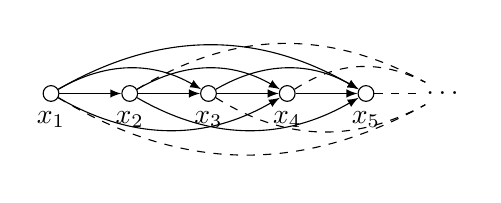
\begin{tikzpicture}
    [
    point/.style={circle,draw,inner sep=0pt,minimum size=2mm},
    collection/.style={thick,rectangle,draw,inner sep=0pt,minimum height=14mm, minimum width= 9mm}
    ]
    \node (1) at (0,1) [point,label=below:$x_1$] {};
    \node (2) at (1,1) [point,label=below:$x_2$] {};
    \node (3) at (2,1) [point,label=below:$x_3$] {};
    \node (4) at (3,1) [point,label=below:$x_4$] {};
    \node (5) at (4,1) [point,label=below:$x_5$] {};
    \node (6) at (5,1) [] {$\dots$};
    \draw [-latex] (1) to (2);
    \draw [-latex] (2) to (3);
    \draw [-latex] (3) to (4);
    \draw [-latex] (4) to (5);
    \draw [dashed] (5) to (6);
    \draw [-latex, bend left] (1) to (3);
    \draw [-latex, bend left] (2) to (4);
    \draw [-latex, bend left] (3) to (5);
    \draw [dashed, bend left] (4) to (6);
    \draw [-latex, bend right] (1) to (4);
    \draw [-latex, bend right] (2) to (5);
    \draw [dashed, bend right] (3) to (6);
    \draw [-latex, bend left] (1) to (5);
    \draw [dashed, bend left] (2) to (6);
    \draw [dashed, bend right] (1) to (6);
  \end{tikzpicture}
\]
Since there exist no two numbers $x,y \in \mathbb{N}$ such that $x < y$ and $y < x$, we get that the Yablo graph indeed is acyclic\todo{This is a bit over-simplified}.
Furthermore, since any natural number has infinitely many numbers strictly larger than it, we get that all the vertices are infinitely branching, making the Yablo graph infinitary (not finitary).

The corresponding discourse theory of the Yablo graph would -- informally -- be the situation with an infinite number of statements, all saying "Every statement after this statement is false".

We will later show that this graph is indeed without a kernel, but for now we will take Yablo's word \cite{analysis-yablo} for it.

One thing should be mentioned at this point; neither odd cycles nor infinitely branching vertices \textit{entails} that their respective graphs are paradoxical.
The two following graphs illustrate this point:
\begin{align}
  \begin{aligned}
    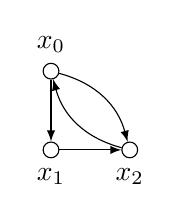
\begin{tikzpicture}
      [
      point/.style={circle,draw,inner sep=0pt,minimum size=2mm},
      collection/.style={thick,rectangle,draw,inner sep=0pt,minimum height=14mm, minimum width= 9mm}
      ]
      \node (0) at (0,1) [point,label=above:$x_0$] {};
      \node (1) at (0,0) [point,label=below:$x_1$] {};
      \node (2) at (1,0) [point,label=below:$x_2$] {};
      \draw [-latex] (0) to (1);
      \draw [-latex] (1) to (2);
      \draw [-latex, bend left] (2) to (0);
      \draw [-latex, bend left] (0) to (2);
    \end{tikzpicture}
  \end{aligned}
\end{align}
The above graph contains an odd cycle, but the singleton set $\{x_2\}$ is a kernel.
\begin{align}
  \begin{aligned}
    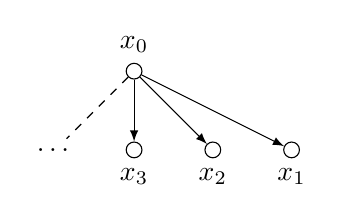
\begin{tikzpicture}
      [
      point/.style={circle,draw,inner sep=0pt,minimum size=2mm},
      collection/.style={thick,rectangle,draw,inner sep=0pt,minimum height=14mm, minimum width= 9mm}
      ]
      \node (0) at (1,2) [point,label=above:$x_0$] {};
      \node (1) at (3,1) [point,label=below:$x_1$] {};
      \node (2) at (2,1) [point,label=below:$x_2$] {};
      \node (3) at (1,1) [point,label=below:$x_3$] {};
      \node (4) at (0,1) [] {$\dots$};
      \draw [-latex] (0) to (1);
      \draw [-latex] (0) to (2);
      \draw [-latex] (0) to (3);
      \draw [dashed] (0) to (4);
    \end{tikzpicture}
  \end{aligned}
\end{align}
The above graph has an infinitely branching vertex $x_0$, but the infinite set $\{x_i \;|\; x > 0\}$ is a kernel.

It is shown that every digraph (with at least one edge) can be transformed into a infinitary dag\footnote{Directed acyclic graph} such that $\alpha$ is a solution to the created dag if and only if it is a solution to the original digraph \cite{apal-digraph}.
This means that for any finitary graph that is paradoxical by the virtue of having an odd cycle, there is an infinitary, \textit{acyclic} digraph that is also paradoxical.
Furthermore, if one is trying to find ways to identify paradoxical graphs, one does only need to look at dags.
The reason for this is simple; say you have a method of identifying paradoxical dags.
Then given any graph, you will be able to decide whether or not it is paradoxical.
If it is a dag, you use your method.
If it is cyclic, translate it, then use your method.
Since the translation preserves and reflects the solutions, one can be sure that the cyclic graph is paradoxical if and only if the resulting dag was paradoxical.

This result will be of great importance to us, enabling us to look only at dags when searching for paradoxes.

	% !TEX root= ../main.tex
\externaldocument{kernelthoery}
\subsection{Dags without kernels}
\label{sub:Dags without kernels}
Knowing that any graph can translate to an equisatisfiable dag, the challenge is now to find sufficient conditions for dags to have kernels, even weaker than the one proved by Richardson (the fact that any finitary dag has a kernel is a direct consequence of Richardson's Theorem).

Michał Walicki has proposed the following thesis:
\begin{align}
  \textit{If a dag has no kernel then it has a ray with infinitely many vertices dominating it.}
\end{align}
Some terminology:
A ray is an infinite sequence of unique vertices $x_0, x_1, x_2, \dots$ such that any two consecutive vertices $x_i,x_i+1$ are connected by the edge$\langle x_i,x_{i+1} \rangle$.
A vertex is dominating a ray if it has infinitely many disjoint paths to it.

The contrapositive of Walicki's thesis suggests a weaker condition for a kernel, since a dag having a ray with infinitely many vertices dominating it implies that the dag is infinitary.

	% !TEX root= ../main.tex
\externaldocument{discoursegraphs}
\externaldocument{kerneltheory}
\section{Resolving GNF-theories}
\label{sec:Resolving GNF-theories}
In this section, we will be presenting an inference system introduced by Walicki in \cite{} which handles clausal theories induced from GNF-theories.

Recall that a thoeory written in GNF has formulae of the following form:
\begin{align}
  x \lar \bigwedge_{i \in I_x} \neg y_i
\end{align}
Using simple operations only, one can manipulate these formulae into an equivalent set of clauses.
We start by writing the above bi-implication as two implications:
\begin{align}
  x \rightarrow \bigwedge_{i \in I_x} \neg y_i \quad\quad \text{and} \quad\quad x \leftarrow \bigwedge_{i \in I_x} \neg y_i
\end{align}
The first implication can be rewritten in the following way:
\begin{align}
  x \rightarrow \bigwedge_{i \in I_x} \neg y_i
  \quad=\quad \neg x \vee \bigwedge_{i \in I_x} \neg y_i
  \quad=\quad \bigwedge_{i \in I_x} (\neg x \vee \neg y_i)
  \quad=\quad \bigwedge_{i \in I_x} \neg (x \wedge y_i)
\end{align}
The second implication can be rewritten in the following way:
\begin{align}
  x \leftarrow \bigwedge_{i \in I_x} \neg y_i
  \quad=\quad x \vee \neg \left( \bigwedge_{i \in I_x} \neg y_i \right)
  \quad=\quad x \vee \bigvee_{i \in I_x} y_i
\end{align}
By splitting the conjunction from the first implication up into individual clauses, we get the following two kinds of clauses for every variable $x$ in the GNF theory:
\begin{align}
  \text{OR-clause:}&\quad x \vee \bigvee_{i \in I_x} y_i\\
  \text{NAND-clauses:}&\quad \neg (x \wedge y_i)\text{, for every }i \in I_x
\end{align}
We will treat both the OR-clauses and the NAND-clauses as sets of atoms, denoting NAND-clauses $\neg (x \wedge y)$ as $\overline{xy}$ and OR-clauses $x \vee y_1 \vee y_2 \vee y_3$ as $xy_1y_2y_3$.
This enables us to state things like $\overline{xy} \subset \overline{xyz}$.
A theory will -- as expected -- be a set of clauses.

If we interpret the initial GNF-theory as a graph $\mathbf{G}=\langle G,N\rangle$, for every vertex $x \in G$, there will be one OR-clause $\{ x \} \cup N(x)$ and for every edge $\langle x,y \rangle \in N$ there will be a NAND-clause $\overline{xy}$.
The graphs from Example~\ref{ex:3graphs} will have the following clausal theories:
\begin{align}
  \mathcal{T}(\mathbf{G_1}) &= \{ a, \ol{a} \}\\
  \mathcal{T}(\mathbf{G_2}) &= \{ abc, b, c, \ol{ab}, \ol{ac} \}\\
  \mathcal{T}(\mathbf{G_3}) &= \{ abc, bc, \ol{ab}, \ol{bc} \}
\end{align}
Further notation: $A\subseteq G$ denotes an OR-clause while $\ol{A} \subseteq G$ denotes a NAND-clause.
Given a graph $\mathbf{G}=\langle G,N\rangle$, we denote the set of all NAND-clauses induced from the graph as NAND and all induced OR-clauses as OR.
The combined set $\Gamma = NAND + OR$ will be our initial clauses in the inference system.
\subsection{The inference system}
\label{sub:The inference system}
We consider the following inference system, but we will focus mainly on proofs using the Axioms together with the (Rneg) rule.
\begin{align}
  \text{(Ax)} &\quad \Gamma \vdash C, \quad \text{for } C \in \Gamma\\
  \text{(Rneg)} &\quad \frac{ \{ \Gamma \vdash \ol{a_iA_i} \; |\; i \in I \} \quad \Gamma \vdash \{ a_i \; |\; i \in I \} }{ \Gamma \vdash \ol{\bigcup_{i \in I} A_i} }\\
  \text{(Rpos)} &\quad \frac{ \Gamma \vdash A \quad \{\Gamma \vdash B_iK_i \; |\; i \in I \} \quad \{ \Gamma \vdash \ol{a_ik} \; |\; i \in I, k \in K_i \} }{ \Gamma \vdash (A \setminus \{ a_i \; |\; i \in I \} ) \cup \bigcup_{i \in I} B_i }
\end{align}
(Rneg) is creating NAND-clauses from NAND-clauses using OR as a side-condition.
(Rpos) is creating OR-clauses from OR-clauses using NAND as a side-condition.
In (Rneg), $\ol{a_iA_i}$ denotes the NAND $\ol{\{ a_i \} \cup A_i}$ with a potentially empty $A_i$.

The premise of the (Rneg) rule is a set of $I$ NAND-clauses together with one OR-clause with $I$ elements such that each atom $a_i$ in the OR-clause is contained within a NAND-clause, and such that each NAND-clause contains an atom from the OR-clause.
The correspondence between the NAND-clauses and the elements of the OR-clause should in other words be bijective.
The conclusion is the union of all the NAND-clauses without their corresponding atom from the OR-clause.

Here are some examples of incorrect applications of the (Rneg)-rules, followed by some correct applications:
\begin{align}
  (1)\;\;\frac{\ol{ax}\quad\ol{by}\quad\ol{cz}}{\ol{xyz}}abx\quad\quad
  (3)\;\;\frac{\ol{ax}\quad\ol{by}}{\ol{xy}}abx\quad\quad
  (2)\;\;\frac{\ol{ax}\quad\ol{by}\quad\ol{bz}}{\ol{xyz}}abx
\end{align}
(1) is incorrect because the NAND $\ol{cz}$ contains no atoms from the OR $abx$.
(2) is incorrect because the number of NAND-clauses does not match the length of the OR-clause.
(3) is incorrect because there exist no bijective correspondence of the type described above.
\begin{align}
  (4)\;\;\frac{\ol{ax}\quad\ol{by}\quad\ol{cz}}{\ol{xyz}}abc\quad\quad
  (5)\;\;\frac{\ol{ax}\quad\ol{b}}{\ol{x}}ab\quad\quad
  (6)\;\;\frac{\ol{ax}\quad\ol{by}\quad\ol{xyz}}{\ol{xyz}}abx
\end{align}
The three above applications are all correct, since all the atoms in each OR-clause get matched to exactly one NAND-clause in such a way that no NAND-clause stays unmatched.

We set no restrictions on the number and cardinality of our clauses, meaning that there might be an infinite number of clauses, and both the OR-clausess and the NAND-clauses might be either finite or infinite in size.
Note that an infinite graph gives infinitely many NAND-clauses, while an infinitary graph also gives us infinitely long OR-clauses.

We study the refutation system that arises from the Axioms and the (Rneg)-rule, calling it Neg.
It is shown in the submitted paper \cite{michal-completeness} that Neg is sound and refutationally complete for theories with only a countable number of OR-clauses.
Soundness gives us that proving $\ol{C}$ for any $C \subseteq G$ implies that the vertices in $C$ cannot all be assigned 1 in the graph model.
Refutational completeness gives us that whenever a graph/theory is inconsistent, we are able to prove $\emptyset$ in Neg.

\subsection{Inconsistency of the Yablo-graph}
\label{sub:Inconsistency of the Yablo-graph}
The inconsistency of the Yablo-graph is easily provable using Neg only.
Since every vertex $x_i$ (using the notation from Figure~\ref{fig:yablo-graph}) has an edge to each vertex $x_j$ where $j > i$, we get that every pair of distinct vertices is connected by an edge.
This means that our set of axioms from the Yablo-graph looks like this:
\begin{align}
  \text{NAND} = \{ \ol{x_ix_j} \; |\; i < j\}
  \quad\quad\quad
  \text{OR} = \{ x_ix_{i+1}x_{i+2}\dots \; |\; i \in \mathbb{N}\}
\end{align}
For any vertex $x_i$ from the Yablo-graph, we are now able to prove $\ol{x_i}$ in the following way:
\begin{prooftree*}
  \Hypo{\ol{x_ix_{i+1}}}
  \Hypo{\ol{x_ix_{i+2}}}
  \Hypo{\ol{x_ix_{i+3}}}
  \Hypo{\dots}
  \Infer4[$x_ix_{i+1}x_{i+2}\dots$]{\ol{x_i}}
\end{prooftree*}
Proving $\emptyset$ is now simple:
\begin{prooftree*}
  \Hypo{\dots}
  \Infer1{\ol{x_1}}
  \Hypo{\dots}
  \Infer1{\ol{x_2}}
  \Hypo{\dots}
  \Infer1{\ol{x_3}}
  \Hypo{\dots}
  \Infer4[$x_1x_2x_3\dots$]{\emptyset}
\end{prooftree*}
A less trivial inconsistency proof is the one on the \textit{Stretched Yablo-graph}.
This proof can be found in the appendix together with the definition of Stretched Yablo.

It is worth mentioning that even though our focus has been -- and will be -- on theories originating from graphs, the results on soundness and completeness holds for any theory consisting of a set of NANDs and a set of ORs.

An example of this is the pigeonhole problem which easily can be represented as a set of NANDs and ORs, but does not directly correspond to a graph (it can of course be translated to a graph theory, like any other propositional theory).
Proofs in Neg of pigeonhole problems of different size are to be found in the appendix\todo{some reference system needed}.

	% !TEX root= ../main.tex
\section{This thesis}
\label{sec:This thesis}
\subsection{Motivation}
\label{sub:Motivation}
Having that (Neg) is both sound and refutationally complete, results linking inconcistency proofs in (Neg) to structures in graphs is of great interest to us, since it can potentially further weaken the current conditions we have for kernels in graphs.
This thesis will thus be concerned mainly with two kinds of questions;
\begin{enumerate}
  \item Are there any characterizing qualities of the proof system (Neg), potentially under certain restrictions?
  \item If the axioms come from a graph, are there any provable results in (Neg) that correspond to certain structures in the graph?
\end{enumerate}
The first question covers qualities like proof length (complexity), size and number of clauses used throughout a proof, the existence of certain clauses in certain proofs, or maybe even the existence of an entire proof normal form.
For instance, an answer to the following question could be of great interest to us: ``Are there certain kinds of clauses that needs to be present in a proof in order to prove $\emptyset$?''.

The second question covers questions like ``What does it mean for the graph that its axioms can prove $\emptyset$?''.
Of course, we know the answer to this question, it means that the graph has no kernel (by soundness of (Neg)).
But what about the provability of $\ol{x}$ for a node $x$ in the graph?
What does that mean for the graph and the node $x$?

Finding a type of clause neccesarily present in an inconsistency proof, together with results on the graph-structural counterpart of that type of clause, gives us in combination a graph-structure neccesarily present in a kernel-free graph (by soundness of (Neg)).
\subsection{Thesis Overview}
\label{sub:Thesis Overview}
THIS SECTION IS NOT UP TO DATE WITH THE FOLLOWING CHAPTERS
Section 2 will take a look at the potential to control the size of NAND-clauses in an inconsistency proof without any restrictions on the axioms.
Section 3 will study the same potential as above, but with graph-based axioms.
We are in both cases above particularly concerned with whether we are able to restrict our proofs to only use binary NAND-clauses.
Section 4 will explore the graph structure that corresponds to unary and binary NAND-clauses, and explain their potential importance.

	\chapter{NAND-clauses in graphs}
	\label{chap:NAND-clauses in graphs}
	% !TEX root= ../main.tex
In this chapter we will motivate and conduct the search for graph structural equivalents of unary and binary NAND-clauses proven in Neg.
An actual graph structure corresponding to the NAND-clauses will not be presented, but we will show some graph structures implying certain provable NAND-clauses.
\begin{definition}
  A clause is \textit{unary} if it contains only one atom.
  A clause is \textit{binary} if it consists of one or two atoms.\todo{should both lengths be included?}
\end{definition}

	% !TEX root= ../main.tex
\section{Motivation}
\label{sec:Motivation}
Since our proof system, Neg, has only one rule, the last step of any inconsistency proof will always look the same:\par
\begin{figure}[!h]
  \centering
  \begin{prooftree*}
    \Hypo{\ol{x_1}}
    \Hypo{\ol{x_2}}
    \Hypo{\ol{x_3}}
    \Hypo{\dots}
    \Infer4[$x_1x_2x_3\dots$]{\varnothing}
  \end{prooftree*}
  \caption{}
  \label{fig:proof_unary_nand}
\end{figure}
The premise will always consist of a collection of NAND-clauses, each of length 1, together with an OR-clause equal to the union of all the NAND-clauses.
It is easy to see that none of the NAND-clauses can be larger than unary, since that would result in a non-empty NAND-clause in the conclusion.
The OR-clause has to equal the union of the NAND-clauses simply by definition of the (RNeg)-rule.

This fact was also observed and formalized by Walicki\cite{michal-completeness}:
\begin{align}
  \Gamma \vdash \{\} \Leftrightarrow \exists K \in \text{OR}: (\forall  k \in K: \Gamma \vdash \ol{k})
\end{align}
We know from the definition that any OR-clause used in the proof system corresponds to a single vertex with its successors in the graph.
We do however not know what the NAND-clauses of length 1 might correspond to.
Knowing this would, by soundness and completeness of Neg, give us the graph structure needed for a kernel not to exist.
\todo{Currently brushing over the restrictions set to the proofs of completeness and soundness. Will fix this later.}

The only thing we \textit{do} know about unary NAND-clauses is that they correspond to vertices that are assigned 0 in all models of the graph.
We get this from soundness of Neg.
This is however not the graph structural property we are ultimately looking for, but we can at least say that we have reduced the question ``What does an inconsistent graph look like?'' to the question ``What does a provably false vertex look like?''.

So what does a unary NAND-clause proven in Neg correspond to in the graph?
Similarly to a proof of $\varnothing$, there is really just one way to prove a unary NAND-clause:\par
\begin{figure}[!h]
  \centering
  \begin{prooftree*}
    \Hypo{\ol{xy_1}}
    \Hypo{\ol{xy_2}}
    \Hypo{\dots}
    \Hypo{\ol{y_n}}
    \Hypo{\ol{y_{n+1}}}
    \Hypo{\dots}
    \Infer6[$y_1y_2\dots y_ny_{n+1}\dots$]{\ol{x}}
  \end{prooftree*}
  \caption{}
  \label{fig:proof_unary_nand}
\end{figure}
Any derivation of a unary NAND-clause $\ol{x}$ must end with a rule application using $K \in \text{OR}$ where for each $k \in K$, there is a NAND-clause in the premise that is either unary, $\ol{k}$ or binary, $\ol{xk}$.
In addition, we require the premise to contain at least one binary NAND-clause, in order to actually be able to conclude with $\ol x$ and not $\varnothing$.

We formalize this observation in the following way:
\begin{align}
  \Gamma \vdash \ol{x} \Leftrightarrow \exists K \in \text{OR}:
  \left ( \begin{tabular}{l}
  $\exists k \in K: G \vdash \ol{kx} \; \wedge$\\
  $\forall k \in K: G \vdash \ol{kx} \vee G \vdash \ol{k}$
  \end{tabular} \right )
\end{align}
Just as we reduced the problem of inconsistency to the problem of unary NAND-clauses, we are able to reduce the problem further to binary NAND-clauses.
We could even continue the reduction further to ternary clauses, quaternary clauses and so on, but without a change of strategy at some point, this seems pointless.

Our current reduction lets us ask how two vertices $x,y$ are \textit{connected} in the graph when their binary NAND $\ol{xy}$ is proven in Neg.
Observe that we have parts of this correspondence down already, with our axioms being all binary.
Vertices directly connected by an edge must therefore be a part of the corresponding graph structure.
%Finding some graph strucural relation that corresponds to binary NAND-clauses might also give us some knowledge about a potential standard form of binary-NAND-proofs.\todo{does this make sense?}

Let $R(a,b)$ denote the existence of some graph structure $R$ between the vertices $a$ and $b$ in some graph $G$; our correspondence can now be formally defined as follows:
\begin{align}
  (1) \quad R(a,b) \quad \Rightarrow \quad G \vdash \ol{ab}\\
  (2) \quad R(a,b) \quad \Leftarrow \quad G \vdash \ol{ab}
\end{align}
The two implications will be referred to as \textit{implication (1)} and \textit{implication (2)}, respectively.

Suppose we manage to find a structure $R$ that satisfied both above implications.
The following equation tells us how that would directly give us a predicate deciding whether or not the graph has a kernel.\todo{This should be rewritten.}
\begin{align}
  &Sol(G) = \varnothing\\
  \Leftrightarrow\; &G \vdash \varnothing\\
  \overset{2.1}{\Leftrightarrow}\;&\exists K \in \text{OR}: (\forall  k \in K: G \vdash \ol{k})\\
  \overset{2.2}{\Leftrightarrow}\;&\exists K \in \text{OR}: (\forall  k \in K: ( \exists L \in \text{OR}:
  \left ( \begin{tabular}{l}
  $\exists l \in L: G \vdash \ol{lk} \; \wedge$\\
  $\forall l \in L: G \vdash \ol{lk} \vee G \vdash \ol{l}$
  \end{tabular} \right ) ) )\\
  \overset{2.3}{\underset{2.4}{\Leftrightarrow}}\;&\exists K \in \text{OR}: (\forall  k \in K: ( \exists L \in \text{OR}:
  \left ( \begin{tabular}{l}
  $\exists l \in L: G \vdash R(l,k) \; \wedge$\\
  $\forall l \in L: G \vdash R(l,k) \vee G \vdash R(l,l)$
  \end{tabular} \right ) ) )
\end{align}
The next sections will present various graph structures, each satisfying implication (1).
Each presented structure will be a generalization of the previous one, ultimately aiming to find a structure general enough to satisfy both implication (1) and implication (2).
Such a structure would be the true graph structural equivalent of a binary NAND provable in Neg.
We did however not manage to find such a graph structure in this thesis.

For each structure presented, implication (1) will be shown, followed by an example disproving implication (2).
The counterexamples will be graphs with the presented structure absent, but with the corresponding NAND-clause still provable.

	% !TEX root= ../main.tex
\section{Odd paths}
\label{sec:Odd paths}
Given two vertices $x_1$ and $x_2$ in a graph $G$, if we in Neg are able to prove $\ol{x_1x_2}$ from the axioms we get from $G$, we say that $x_1$ and $x_2$ are \textit{vel-connected}.
This section will try to answer the question ``what kind of graph structures imply that certain vertices are vel-connected?''.

Because of soundness of Neg, if two vertices are vel-connected in a graph, for any kernel $K$ in that graph, at least one of the two vertices are outside $K$.
The counterpositive of this observation being that for a graph $G$, if there exists a kernel $K \subseteq G$ such that two vertices, $x_1$ and $x_2$ are both in $K$, then $x_1$ and $x_2$ cannot be vel-connected in $G$.
This fact will be used when arguing why some graph structures are \textit{not} giving us vel-connected vertices.

We already know that whenever two vertices are connected by an edge, their binary NAND is trivially provable in Neg, since it is a part of the axioms.

We illustrate this case with the figure below, where dashed lines represent possible out-edges to irrelevant parts of the graph.
If a vertex has no dashed edges, it means that we disallow any additional edges out from this vertex.
\[
  \begin{tikzpicture}
    [
    point/.style={circle,draw,inner sep=0pt,minimum size=2mm},
    ]
    \node (1) at (1,1) [point] {};
    \node (2) at (2,1) [point] {};
    \draw [-latex] (1) to (2);

    \node (e1) [above left=4mm and 6mm of 1]  {};
    \node (e2) [left=8mm of 1] {};
    \node (e3) [below left=4mm and 6mm of 1] {};
    \node (e4) [above right=4mm and 6mm of 2] {};
    \node (e5) [right=8mm of 2] {};
    \node (e6) [below right=4mm and 6mm of 2] {};
    \draw [dashed] (e1) to (1);
    \draw [dashed] (e2) to (1);
    \draw [dashed] (e3) to (1);
    \draw [dashed] (e4) to (2);
    \draw [dashed] (e5) to (2);
    \draw [dashed] (e6) to (2);
  \end{tikzpicture}
\]
The basic example above tells us that two vertices are vel-connected when one is the successor of the other.
It is however easy to find a case examplifying how the implication does not hold in the opposite direction.
\[
  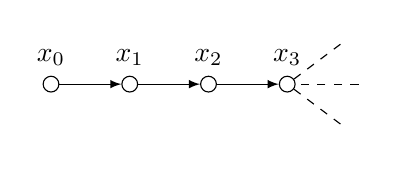
\begin{tikzpicture}
    [
    point/.style={circle,draw,inner sep=0pt,minimum size=2mm},
    ]
    \node (1) at (0,1) [point,label=above:$x_0$] {};
    \node (2) at (1,1) [point,label=above:$x_1$] {};
    \node (3) at (2,1) [point,label=above:$x_2$] {};
    \node (4) at (3,1) [point,label=above:$x_3$] {};
    \draw [-latex] (1) to (2);
    \draw [-latex] (2) to (3);
    \draw [-latex] (3) to (4);

    \node (e4) [above right=4mm and 6mm of 4] {};
    \node (e5) [right=8mm of 4] {};
    \node (e6) [below right=4mm and 6mm of 4] {};
    \draw [dashed] (e4) to (4);
    \draw [dashed] (e5) to (4);
    \draw [dashed] (e6) to (4);
  \end{tikzpicture}
\]
The above graph provides us the following axioms:
$NAND = \{\ol{x_0x_1},\ol{x_1x_2},\ol{x_2x_3}\}$, $OR = \{x_0x_1,x_1x_2,x_2x_3\}$.
From these axioms, we can now, despite the fact that the vertices $x_0$ and $x_3$ are not connected by an edge, easily prove the NAND-clause $\ol{x_0x_3}$:

\begin{prooftree*}
  \Hypo{\ol{x_0x_1}}
  \Hypo{\ol{x_2x_3}}
  \Infer[left label=$x_1x_2$]2{\ol{x_0x_3}}
\end{prooftree*}

Intuitively, one can imagine that the proof above is connecting two NAND-clauses using an OR-clause, resulting in a new binary NAND-clause containing vertices that are weaklier connected than the ones we started with.
This can be done repeatedly, resulting in the ability to prove binary NAND-clauses from vertices that are connected by arbitrarily long paths of the kind above.

Consider the following graph:
\[
  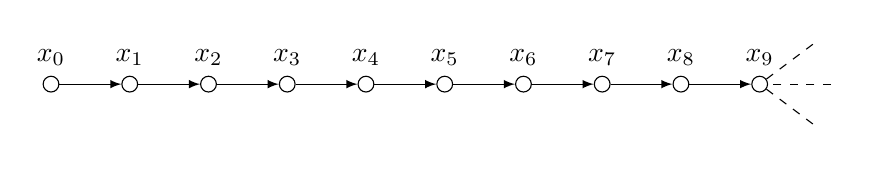
\begin{tikzpicture}
    [
    point/.style={circle,draw,inner sep=0pt,minimum size=2mm},
    ]
    \node (1) at (0,1) [point,label=above:$x_0$] {};
    \node (2) at (1,1) [point,label=above:$x_1$] {};
    \node (3) at (2,1) [point,label=above:$x_2$] {};
    \node (4) at (3,1) [point,label=above:$x_3$] {};
    \node (5) at (4,1) [point,label=above:$x_4$] {};
    \node (6) at (5,1) [point,label=above:$x_5$] {};
    \node (7) at (6,1) [point,label=above:$x_6$] {};
    \node (8) at (7,1) [point,label=above:$x_7$] {};
    \node (9) at (8,1) [point,label=above:$x_8$] {};
    \node (10) at (9,1) [point,label=above:$x_9$] {};
    \draw [-latex] (1) to (2);
    \draw [-latex] (2) to (3);
    \draw [-latex] (3) to (4);
    \draw [-latex] (4) to (5);
    \draw [-latex] (5) to (6);
    \draw [-latex] (6) to (7);
    \draw [-latex] (7) to (8);
    \draw [-latex] (8) to (9);
    \draw [-latex] (9) to (10);

    \node (e4) [above right=4mm and 6mm of 10] {};
    \node (e5) [right=8mm of 10] {};
    \node (e6) [below right=4mm and 6mm of 10] {};
    \draw [dashed] (e4) to (10);
    \draw [dashed] (e5) to (10);
    \draw [dashed] (e6) to (10);
  \end{tikzpicture}
\]

With axioms from the above graph, $\ol{x_0x_9}$ can be proven in Neg in the following way:

\begin{prooftree*}
  \Hypo{\ol{x_0x_1}}
  \Hypo{\ol{x_2x_3}}
  \Infer[left label=$x_1x_2$]2{\ol{x_0x_3}}
  \Hypo{\ol{x_4x_5}}
  \Infer[left label=$x_4x_5$]2{\ol{x_0x_5}}
  \Hypo{\ol{x_6x_7}}
  \Infer[left label=$x_6x_7$]2{\ol{x_0x_7}}
  \Hypo{\ol{x_8x_9}}
  \Infer[left label=$x_8x_9$]2{\ol{x_0x_9}}
\end{prooftree*}

Observe that the above proof is also proving $\ol{x_0x_3}$, $\ol{x_0x_5}$ and $\ol{x_0x_7}$ along the way, all of which contain vertices connected by paths of \textit{odd} length.
This is an important point.
NAND-clauses containing vertices connected only by paths of \textit{even} length cannot be proven in the same manner as above.

In many cases, such NAND-clauses cannot be proven at all.
This is examplified by the below graph, with a kernel containing the vertices $a$ and $b$, showing that the NAND $\ol{ab}$ is unprovable in Neg.
The kernel in the graph below is represented by the black vertices.

\[
  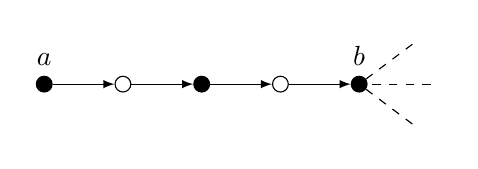
\begin{tikzpicture}
    [
    point/.style={circle,draw,inner sep=0pt,minimum size=2mm},
    one/.style={fill=black},
    ]
    \node (1) at (0,1) [point, one, label=above:$a$] {};
    \node (2) at (1,1) [point] {};
    \node (3) at (2,1) [point, one] {};
    \node (4) at (3,1) [point] {};
    \node (5) at (4,1) [point, one, label=above:$b$] {};
    \draw [-latex] (1) to (2);
    \draw [-latex] (2) to (3);
    \draw [-latex] (3) to (4);
    \draw [-latex] (4) to (5);

    \node (e4) [above right=4mm and 6mm of 5] {};
    \node (e5) [right=8mm of 5] {};
    \node (e6) [below right=4mm and 6mm of 5] {};
    \draw [dashed] (e4) to (5);
    \draw [dashed] (e5) to (5);
    \draw [dashed] (e6) to (5);
  \end{tikzpicture}
\]

Restricting our paths to be of odd length lets us avoid cases like the one above, but there are still some cases left to avoid, in order for our implication to hold.

All the paths so far have been free for any branching, i.e. all vertices in the paths have been of degree 1.
We will call such paths \textit{fully trimmed paths}, and formally define them as paths where for each pair of vertices $x$ and $y$ consecutive in the path, $N(x) = \{y\}$.

If two vertices $a$ and $b$ are connected by an odd path that is \textit{not} fully trimmed, $\ol{ab}$ is not neseccarily provable in Neg.
The below graph examplifies this with a kernel containing both $a$ and $b$.

\[
  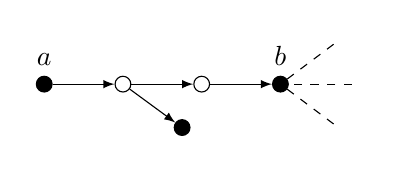
\begin{tikzpicture}
    [
    point/.style={circle,draw,inner sep=0pt,minimum size=2mm},
    one/.style={fill=black},
    ]
    \node (1) at (0,1) [point, one, label=above:$a$] {};
    \node (2) at (1,1) [point] {};
    \node (2b) [point, one, below right=4mm and 6mm of 2] {};
    \node (3) at (2,1) [point] {};
    \node (4) at (3,1) [point, one,label=above:$b$] {};
    \draw [-latex] (1) to (2);
    \draw [-latex] (2) to (3);
    \draw [-latex] (2) to (2b);
    \draw [-latex] (3) to (4);

    \node (e4) [above right=4mm and 6mm of 4] {};
    \node (e5) [right=8mm of 4] {};
    \node (e6) [below right=4mm and 6mm of 4] {};
    \draw [dashed] (e4) to (4);
    \draw [dashed] (e5) to (4);
    \draw [dashed] (e6) to (4);
  \end{tikzpicture}
\]

Generalizing this, we get that whenever two vertices, $x_0$ and $x_k$, are connected by a fully trimmed path of odd length, they are vel-connected.
Their corresponding NAND-clause $\ol{x_0x_k}$ can be proven in Neg in the following way:
\begin{prooftree*}
  \Hypo{\ol{x_0x_1}}
  \Hypo{\ol{x_2x_3}}
  \Infer[left label=$x_1x_2$]2{\ol{x_0x_3}}
  \Hypo{\ol{x_4x_5}}
  \Infer[left label=$x_3x_4$]2{\ol{x_0x_5}}
  \Ellipsis{}{\ol{x_0x_{k-2}}}
  \Hypo{\ol{x_{k-1}x_k}}
  \Infer[left label=$x_{k-2}x_{k-1}$]2{\ol{x_0x_k}}
\end{prooftree*}

All the OR-clauses used are indeed binary, letting us prove our NAND-clause without introducing any other clauses than the ones we get from the path itself.
However, notice that only half of the OR-clauses is actually in use in such a proof.
Thus, we need only to restrict half of the vertices in the path to not branch.

With the above proof in mind, consider the following graph:
\[
  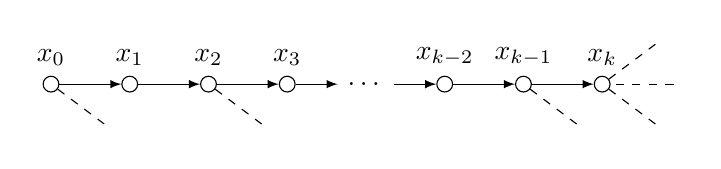
\begin{tikzpicture}
    [
    point/.style={circle,draw,inner sep=0pt,minimum size=2mm},
    ]
    \node (1) at (0,1) [point,label=above:$x_0$] {};
    \node (2) at (1,1) [point,label=above:$x_1$] {};
    \node (3) at (2,1) [point,label=above:$x_2$] {};
    \node (4) at (3,1) [point,label=above:$x_3$] {};
    \node (dots) at (4,1) [] {\dots};
    \node (k2) at (5,1) [point,label=above:$x_{k-2}$] {};
    \node (k1) at (6,1) [point,label=above:$x_{k-1}$] {};
    \node (k) at (7,1) [point,label=above:$x_k$] {};
    \draw [-latex] (1) to (2);
    \draw [-latex] (2) to (3);
    \draw [-latex] (3) to (4);
    \draw [-latex] (4) to (dots);
    \draw [-latex] (dots) to (k2);
    \draw [-latex] (k2) to (k1);
    \draw [-latex] (k1) to (k);

    \node (e4) [above right=4mm and 6mm of k] {};
    \node (e5) [right=8mm of k] {};
    \node (e6) [below right=4mm and 6mm of k] {};
    \draw [dashed] (e4) to (k);
    \draw [dashed] (e5) to (k);
    \draw [dashed] (e6) to (k);

    \node (b1) [below right=4mm and 6mm of 1] {};
    \node (b3) [below right=4mm and 6mm of 3] {};
    \node (bk1) [below right=4mm and 6mm of k1] {};
    \draw [dashed] (1) to (b1);
    \draw [dashed] (3) to (b3);
    \draw [dashed] (k1) to (bk1);
  \end{tikzpicture}
\]
In the above graph, only every other vertex are restricted to only have one successor.
We will call this path variant an \textit{oddly trimmed path}, and define it formally as follows:
A path $\langle x_0,x_k\rangle$\todo{This notation is not explained} is oddly trimmed if for each odd $i < k$, $N(x_i) = \{x_{i+1}\}$.
One can immediately note that any fully trimmed path is also oddly trimmed.

The axioms we get from the oddly trimmed path above does not differ significantly from the fully trimmed variant.
Since the vertices $x_0, x_2, x_4, \dots ,x_{k_1}$ no longer have single successors, their corresponding OR-clauses will no longer be binary.
However, since none of these OR-clauses are used in the above proof, the proof will remain valid also for the oddly trimmed path.

We can thus generalize further and say that any two vertices connected by an oddly trimmed path of odd length is vel-connected.

	% !TEX root= ../main.tex
\section{Odd vels}
\label{sec:Odd vels}
Consider the following graph:
\[
  \begin{tikzpicture}
    [
    point/.style={circle,draw,inner sep=0pt,minimum size=2mm}
    ]
    \node (x0) at (0,3) [point, label=above:$x_0$] {};
    \node (x1) at (1,2) [point, label=above:$x_1$] {};
    \node (x2) at (2,1) [point, label=above:$x_2$] {};
    \node (x3) at (3,0) [point, label=above:$x_3$] {};
    \node (x4) at (4,1) [point, label=above:$x_4$] {};
    \node (x5) at (5,2) [point, label=above:$x_5$] {};
    \draw [-latex] (x0) to (x1);
    \draw [-latex] (x1) to (x2);
    \draw [-latex] (x2) to (x3);
    \draw [-latex] (x4) to (x3);
    \draw [-latex] (x5) to (x4);

    \node (e1) [below left=6mm and 4mm of x3]  {};
    \node (e2) [below=8mm of x3] {};
    \node (e3) [below right=6mm and 4mm of x3] {};
    \draw [dashed] (e1) to (x3);
    \draw [dashed] (e2) to (x3);
    \draw [dashed] (e3) to (x3);

    \node (b0) [below left=6mm and 4mm of x0] {};
    \node (b2) [below left=6mm and 4mm of x2] {};
    \node (b5) [below right=6mm and 4mm of x5] {};
    \draw [dashed] (x0) to (b0);
    \draw [dashed] (x2) to (b2);
    \draw [dashed] (x5) to (b5);
  \end{tikzpicture}
\]
From the above graph, $x_0x_5$ can be proven in the same way as in the proof of $x_0x_9$ from earlier.
Again, the only thing we are changing in terms of the axioms are the OR-clauses that are not used in the proof.

We will call this kind of graph structure an \textit{odd vel} and define it formally in the following way:
Two vertices $a$ and $b$ have an odd vel between them if there exists a vertex $c$ such that there are oddly trimmed paths from $a$ to $c$ and from $b$ to $c$, one of even length (possibly 0) and one of odd length.

Notice that an oddly trimmed path of odd length is just an instance of an odd vel where the even path is of length 0.

  % !TEX root= ../main.tex
\externaldocument{odd_paths}
\externaldocument{odd_vels}
\section{Generalizing trimming}
\label{sec:Generalizing trimming}
In this section, we will take a closer look at the current concept of trimming, and through some examples introduce a more general definition.
So far, trimming has meant forcing certain vertices to point only at its successor in a path.

In Section~\ref{sec:Odd paths} we motivated the concept of trimmed paths by presenting the graph in Figure~\ref{fig:kernel_untrimmed}.
The figure showed how adding out-edges to certain vertices in the odd path makes the corresponding NAND-clause unprovable.

Notice however that adding a loop on the vertex to which the path branches, leaves us with a different situation.\par
\begin{figure}[!h]
  \centering
  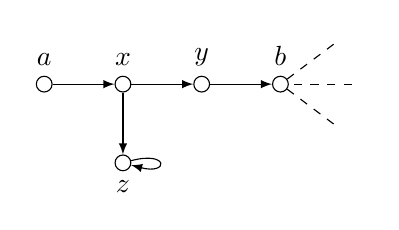
\begin{tikzpicture}
    [
    point/.style={circle,draw,inner sep=0pt,minimum size=2mm},
    one/.style={fill=black},
    ]
    \node (1) at (0,1) [point, label=above:$a$] {};
    \node (2) at (1,1) [point, label=above:$x$] {};
    \node (2b) at (1,0) [point, label=below:$z$] {};
    \node (3) at (2,1) [point, label=above:$y$] {};
    \node (4) at (3,1) [point,label=above:$b$] {};
    \draw [-latex] (1) to (2);
    \draw [-latex] (2) to (3);
    \draw [-latex] (2) to (2b);
    \draw [-latex] (3) to (4);
    \draw [-latex, loop right] (2b) to (2b);

    \node (e4) [above right=4mm and 6mm of 4] {};
    \node (e5) [right=8mm of 4] {};
    \node (e6) [below right=4mm and 6mm of 4] {};
    \draw [dashed] (e4) to (4);
    \draw [dashed] (e5) to (4);
    \draw [dashed] (e6) to (4);
  \end{tikzpicture}
  \caption{}
  \label{fig:path_3_with_loop}
\end{figure}
The addition of the loop adds $\ol{z}$ to the axioms.
The NAND-clause $\ol{ab}$ can now easily be proven in the following way:\par
\begin{figure}[!h]
  \centering
  \begin{prooftree*}
    \Hypo{\ol{ax}}
    \Hypo{\ol{yb}}
    \Hypo{\ol{z}}
    \Infer[left label=$xyz$]3{\ol{ab}}
  \end{prooftree*}
  \caption{}
  \label{fig:proof_loop}
\end{figure}
This shows the fact that vertices at odd positions in a path can indeed branch off to other vertices than their path successor and still contribute to a provable NAND-clause, just as long as the vertices they branch off to satisfy certain criteria.
If the vertex is provably false, we can use that unary NAND-clause, like we did in the above proof, to handle the non-binary OR-clauses.
This observation lets us generalize our definition of trimmed vertices and still have our vel-relation satisfy implication (1).

The new, general notion of trimming can be formally defined like follows:
\begin{definition}
  Given a path and two consecutive vertices $x$ and $y$ from that path, we say that $x$ is \textit{trimmed}, with respect to that path, if $c \in N(x)\setminus y \Rightarrow \Gamma \vdash \ol{c}$.
  \label{def:new_trimming}
\end{definition}
The problem with this generalized definition is that it is using the notion of provability and is thus not a purely graph-structural definition.
This in turn makes our vel-relation no longer a purely graph-structural definition.
With such a definition, whenever we want to check whether two vertices have a vel between them, we may have to work out the actual provability of certain unary NAND-clauses, which is exactly what we try to avoid with our vel-relation.

In addition to this problem, consider the following two graphs:\par
\begin{figure}[h!]
  \centering
  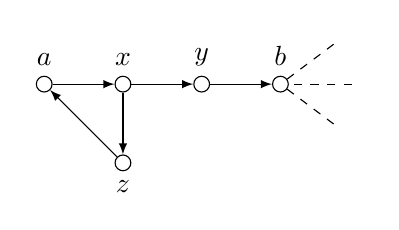
\begin{tikzpicture}
    [
    point/.style={circle,draw,inner sep=0pt,minimum size=2mm},
    one/.style={fill=black}
    ]
    \node (1) at (0,1) [point, label=above:$a$] {};
    \node (2) at (1,1) [point, label=above:$x$] {};
    \node (2b) at (1,0) [point, label=below:$z$] {};
    \node (3) at (2,1) [point, label=above:$y$] {};
    \node (4) at (3,1) [point,label=above:$b$] {};
    \draw [-latex] (1) to (2);
    \draw [-latex] (2) to (3);
    \draw [-latex] (2) to (2b);
    \draw [-latex] (3) to (4);
    \draw [-latex] (2b) to (1);

    \node (e4) [above right=4mm and 6mm of 4] {};
    \node (e5) [right=8mm of 4] {};
    \node (e6) [below right=4mm and 6mm of 4] {};
    \draw [dashed] (e4) to (4);
    \draw [dashed] (e5) to (4);
    \draw [dashed] (e6) to (4);
  \end{tikzpicture}
  \hspace{5mm}
  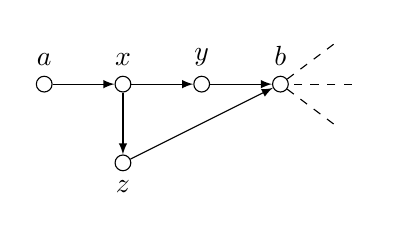
\begin{tikzpicture}
    [
    point/.style={circle,draw,inner sep=0pt,minimum size=2mm},
    one/.style={fill=black},
    ]
    \node (1) at (0,1) [point, label=above:$a$] {};
    \node (2) at (1,1) [point, label=above:$x$] {};
    \node (2b) at (1,0) [point, label=below:$z$] {};
    \node (3) at (2,1) [point, label=above:$y$] {};
    \node (4) at (3,1) [point,label=above:$b$] {};
    \draw [-latex] (1) to (2);
    \draw [-latex] (2) to (3);
    \draw [-latex] (2) to (2b);
    \draw [-latex] (3) to (4);
    \draw [-latex] (2b) to (4);

    \node (e4) [above right=4mm and 6mm of 4] {};
    \node (e5) [right=8mm of 4] {};
    \node (e6) [below right=4mm and 6mm of 4] {};
    \draw [dashed] (e4) to (4);
    \draw [dashed] (e5) to (4);
    \draw [dashed] (e6) to (4);
  \end{tikzpicture}
  \caption{}
  \label{fig:path_3_with_backedges}
\end{figure}
Like with the graph from Figure~\ref{fig:path_3_with_loop}, the above graphs are both based on Figure~\ref{fig:kernel_untrimmed}, each with only one edge added.
The left variant has $\ol{az}$ in its axioms, while the right variant has $\ol{bz}$, again making their respective proofs of $\ol{ab}$ almost trivial.\par
\begin{figure}[!h]
  \centering
  \begin{prooftree}
    \Hypo{\ol{ax}}
    \Hypo{\ol{yb}}
    \Hypo{\ol{za}}
    \Infer[left label=$xyz$]3{\ol{ab}}
  \end{prooftree}
  \hspace{5mm}
  \begin{prooftree}
    \Hypo{\ol{ax}}
    \Hypo{\ol{yb}}
    \Hypo{\ol{zb}}
    \Infer[left label=$xyz$]3{\ol{ab}}
  \end{prooftree}
  \caption{}
  \label{fig:proof_loop}
\end{figure}
\FloatBarrier
The above proofs do not rely on any provably false vertex, but rather make use of the fact that $z$ is connected to one of the vertices contained in the NAND-clause that we are trying to prove.

In the case of Figure~\ref{fig:path_3_with_backedges}, $\ol{ab}$ will be provable as long as for all the successors $z$ of $x$, either $\ol{z}$, $\ol{az}$ or $\ol{bz}$ are provable in Neg.

This means that our definition of trimming should be generalized even further, taking into account the observation made above.
Such a generalization must add the case where, given a vel between $a$ and $b$, trimmed vertices may branch off to a vertex $c$ as long as either $\ol{ac}$ or $\ol{bc}$ are provable in Neg.

In order to keep our definitions strictly graph structural , we change our approach and present two inductive definitions satisfying implication (1).

	% !TEX root= ../main.tex
\externaldocument{odd_paths}
\section{Generalizing trimming}
\label{sec:Generalizing trimming}
In this section, we will take a closer look at the current concept of trimming, and through some examples introduce a more general definition.
So far, trimming has meant forcing certain vertices to point only at its successor in a path.

In Section~\ref{sec:Odd paths} we motivated the concept of trimmed paths by presenting the Figure~\ref{fig:kernel_untrimmed}.
The figure shows how a path that normally provides a provable NAND-clause may be "ruined" by adding out-edges to certain vertices in the path, making certain vital OR-clauses non-binary and thus making the NAND-clause unprovable.

Notice however that adding a loop on the vertex to which the path branches, leaves us with a completely different situation.\par
\begin{figure}[!h]
  \centering
  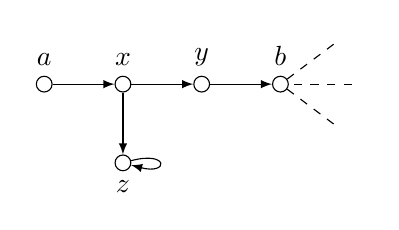
\begin{tikzpicture}
    [
    point/.style={circle,draw,inner sep=0pt,minimum size=2mm},
    one/.style={fill=black},
    ]
    \node (1) at (0,1) [point, label=above:$a$] {};
    \node (2) at (1,1) [point, label=above:$x$] {};
    \node (2b) at (1,0) [point, label=below:$z$] {};
    \node (3) at (2,1) [point, label=above:$y$] {};
    \node (4) at (3,1) [point,label=above:$b$] {};
    \draw [-latex] (1) to (2);
    \draw [-latex] (2) to (3);
    \draw [-latex] (2) to (2b);
    \draw [-latex] (3) to (4);
    \draw [-latex, loop right] (2b) to (2b);

    \node (e4) [above right=4mm and 6mm of 4] {};
    \node (e5) [right=8mm of 4] {};
    \node (e6) [below right=4mm and 6mm of 4] {};
    \draw [dashed] (e4) to (4);
    \draw [dashed] (e5) to (4);
    \draw [dashed] (e6) to (4);
  \end{tikzpicture}
  \caption{}
  \label{fig:path_3_with_loop}
\end{figure}
The addition of the loop adds $\ol{z}$ to the axioms.
The NAND-clause $\ol{ab}$ can now easily be proven in the following way:\par
\begin{figure}[!h]
  \centering
  \begin{prooftree*}
    \Hypo{\ol{ax}}
    \Hypo{\ol{yb}}
    \Hypo{\ol{z}}
    \Infer[left label=$xyz$]3{\ol{ab}}
  \end{prooftree*}
  \caption{}
  \label{fig:proof_loop}
\end{figure}
This shows the fact that vertices at odd positions in a path can indeed branch off to other vertices than their path successor and still contribute to a provable NAND-clause, just as long as the vertices they branch off to are provably false in Neg.
If the vertex is provably false, we can use that unary NAND-clause, like we did in the above proof, to handle the non-binary OR-clauses.
This observation lets us generalize our notion of trimmed vertices.

The big problem with this generalization is that it makes our vel-relation no longer a purely graph-structural one.
With such a definition, whenever we want to check whether two vertices have a vel between them, we may have to work out the actual provability of certain unary NAND-clauses.
This is exactly what we try to avoid with our vel-relation.

To make matters worse, consider the following two graphs:\par
\begin{figure}[h!]
  \centering
  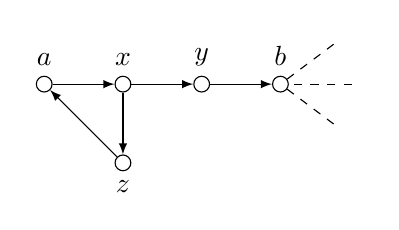
\begin{tikzpicture}
    [
    point/.style={circle,draw,inner sep=0pt,minimum size=2mm},
    one/.style={fill=black},
    ]
    \node (1) at (0,1) [point, label=above:$a$] {};
    \node (2) at (1,1) [point, label=above:$x$] {};
    \node (2b) at (1,0) [point, label=below:$z$] {};
    \node (3) at (2,1) [point, label=above:$y$] {};
    \node (4) at (3,1) [point,label=above:$b$] {};
    \draw [-latex] (1) to (2);
    \draw [-latex] (2) to (3);
    \draw [-latex] (2) to (2b);
    \draw [-latex] (3) to (4);
    \draw [-latex] (2b) to (1);

    \node (e4) [above right=4mm and 6mm of 4] {};
    \node (e5) [right=8mm of 4] {};
    \node (e6) [below right=4mm and 6mm of 4] {};
    \draw [dashed] (e4) to (4);
    \draw [dashed] (e5) to (4);
    \draw [dashed] (e6) to (4);
  \end{tikzpicture}
  \hspace{5mm}
  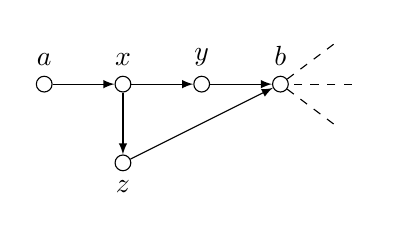
\begin{tikzpicture}
    [
    point/.style={circle,draw,inner sep=0pt,minimum size=2mm},
    one/.style={fill=black},
    ]
    \node (1) at (0,1) [point, label=above:$a$] {};
    \node (2) at (1,1) [point, label=above:$x$] {};
    \node (2b) at (1,0) [point, label=below:$z$] {};
    \node (3) at (2,1) [point, label=above:$y$] {};
    \node (4) at (3,1) [point,label=above:$b$] {};
    \draw [-latex] (1) to (2);
    \draw [-latex] (2) to (3);
    \draw [-latex] (2) to (2b);
    \draw [-latex] (3) to (4);
    \draw [-latex] (2b) to (4);

    \node (e4) [above right=4mm and 6mm of 4] {};
    \node (e5) [right=8mm of 4] {};
    \node (e6) [below right=4mm and 6mm of 4] {};
    \draw [dashed] (e4) to (4);
    \draw [dashed] (e5) to (4);
    \draw [dashed] (e6) to (4);
  \end{tikzpicture}
  \caption{}
  \label{fig:path_3_with_backedges}
\end{figure}
Like with the graph from Figure~\ref{fig:path_3_with_loop}, the above graphs are both based on Figure~\ref{fig:kernel_untrimmed}, each with only one edge added.
The left variant has $\ol{az}$ in its axioms, while the right variant has $\ol{bz}$, again making their respective proofs of $\ol{ab}$ almost trivial.\par
\begin{figure}[!h]
  \centering
  \begin{prooftree}
    \Hypo{\ol{ax}}
    \Hypo{\ol{yb}}
    \Hypo{\ol{za}}
    \Infer[left label=$xyz$]3{\ol{ab}}
  \end{prooftree}
  \hspace{5mm}
  \begin{prooftree}
    \Hypo{\ol{ax}}
    \Hypo{\ol{yb}}
    \Hypo{\ol{zb}}
    \Infer[left label=$xyz$]3{\ol{ab}}
  \end{prooftree}
  \caption{}
  \label{fig:proof_loop}
\end{figure}
\FloatBarrier
The above proofs do not rely on any provably false vertex, but rather make use of the fact that $z$ is connected to one of the vertices contained in the NAND-clause that we are trying to prove.

In the case of Figure~\ref{fig:path_3_with_backedges}, $\ol{ab}$ will be provable as long as for all the successors $z$ of $x$, either $\ol{z}$, $\ol{az}$ or $\ol{bz}$ are provable in Neg.

This means that our concept of trimming needs further weakening, taking into account the observation made above.
Such a weakening will simply add the case where, given a vel between $a$ and $b$, trimmed vertices may branch off to vertices $c$ as long as either $\ol{ac}$ or $\ol{bc}$ are provable in Neg.

The definition now bases the provability of $\ol{ab}$ on the provability of a set of other binary NAND-clauses, suggesting an inductive approach for our definitions.

\section{Inductive definitions}
\label{sec:Inductive definitions}
All the graph structures presented in this chapter so far can easily be defined inductively.
For instance, given some graph $\mathbf{G}=(G,N)$, let $V_1 \subseteq G \times G$ denote the set of all pairs of vertices related by our original vel-definition where trimmed meant strictly non-branching.

We can define $V_1$ inductively in the following way, with $a$ and $b$ being arbitrary vertices from $G$.
\begin{align}
  \textbf{(BC):}&\quad N(a,b) \vee N(b,a) &\Rightarrow  V_1(a,b)\\
  \textbf{(IS):}&\quad \exists c \in N(a): (N(c) =\{d\} \wedge V_1(d,b)) &\Rightarrow V_1(a,b)
\end{align}
The symmetry in the base case is what makes this a definition of a vel and not a path, while the trimmed-ness gets expressed by the restrictions we set on vertex $c$.

Adding the new weaker trimming-restriction is now easy.
Let $V_2 \subseteq G \times G$ be the set of all pairs of vertices related by our new vel-definition.
$V_2$ can now be defined inductively in the following way, again with $a$ and $b$ as arbitrary vertices from $G$.
\begin{align}
  \textbf{(BC):}&\quad N(a,b) \vee N(b,a) &\Rightarrow V_2(a,b)\\
  \textbf{(IS):}&\quad \exists c \in N(a):
  \left ( \begin{tabular}{l}
  $\exists d \in N(c): V_2(d,b) \quad \wedge$\\
  $\forall d \in N(c): V_2(d,b) \vee V_2(d,a) \vee V_2(d,d)$
  \end{tabular} \right )
  &\Rightarrow V_2(a,b)
\end{align}

  % !TEX root= ../main.tex
\section{Concluding remarks}
\label{sec:Concluding remarks}
In the process of repeatedly generalizing our graph structural definitions, we have reached a situation where our current definition is almost identical to the actual axioms and rule-applications in our proof system; more specifically, the applications with binary NAND-clauses in their conclusion.
This comes as no surprise, but is a bit disappointing.
The original goal was to find some graph structual relation $V$, independent of the definition of Neg, such that $V(a,b) \; \Leftrightarrow \; \vdash \ol{ab}$ (implication (1) and (2)).
This would as a result give us a graph structure present only when the graph in question was kernel free.
It has however become apparent that no simple graph structural definition suffices in satisfying these implications.
Even $V_3$ falls short in this endeavour.

	\chapter{Refutational incompleteness of BNeg}
	\label{chap:Refutational incompleteness of BNeg}
	% !TEX root= ../main.tex
In this chapter we will investigate the statement that whenever a theory is inconsistent, it can be proven in Neg using unary and binary NAND-clauses only.
Such a result would be significant both because it would be a strong property for a proof system to have in general, but also because it could potentially help us to further characterize a kernel-free graph.

Having that any inconsistency can be proven in Neg using unary and binary NAND-clauses only, might imply a similar property in kernel-free graphs, namely that inconsistencies can be described as a collection of pairwise structural relations between vertices.

We will check the statement first for non-graph-based theories and then for theories based on graphs with different properties.

	% !TEX root= ../main.tex
\externaldocument{../binary_nands/motivation}
\section{Inconsistencies in general theories}
\label{sec:Inconsistencies in general theories}
This section will show that there exist inconsistent theories such that their inconsistencies are not possible to prove in Neg using binary NAND-clauses only.
We will prove the pigeonhole principle in Neg to exemplify this.

The pigeonhole principle states that whenever you have $n$ pigeons and $m$ holes such that $n > m$, then at least one hole must contain more than one pigeon.
We can prove this principle in Neg by proving an inconsistency of the theory that (1) all $n$ pigeons are contained in a hole and (2) each hole contains only one pigeon.

Letting the atom $x_i$ denote the pigeon $i$ occupying the hole $x$, the above theory, with $n$ pigeons and $m$ holes, can be formalized in the following way:
\begin{align}
  \text{(1):}\quad &\{ \; 1_i2_i3_i\dots m_i \;|\; i \leq n \; \}\\
  \text{(2):}\quad &\{ \; \ol{x_ix_j} \;|\; i < j \leq n, x \leq m \; \}
\end{align}
\subsection{Proving the pigeonhole principle}
\label{sub:Proving the pigeonhole principle}
The pigeonhole principle for 4 pigeons and 3 holes will have the following axioms:
\begin{align}
  \begin{split}
    \text{OR} &= \{ \; 1_12_13_1,\; 1_22_23_2,\; 1_32_33_3,\; 1_42_43_4 \; \}\\
    \text{NAND} &= \left \{
    \begin{tabular}{c}
      $\ol{1_11_2},\;\ol{1_11_3},\;\ol{1_11_4},\;\ol{1_21_3},\;\ol{1_21_4},\;\ol{1_31_4},$\\
      $\ol{2_12_2},\;\ol{2_12_3},\;\ol{2_12_4},\;\ol{2_22_3},\;\ol{2_22_4},\;\ol{2_32_4},$\\
      $\ol{3_12_2},\;\ol{3_13_3},\;\ol{3_13_4},\;\ol{3_23_3},\;\ol{3_23_4},\;\ol{3_33_4}$
    \end{tabular}
    \right \}
  \end{split}
  \label{eq:ax_pigeon}
\end{align}

From the axioms above we can prove inconsistency by first proving the three NAND-clauses $\ol{1_4}$, $\ol{2_4}$ and $\ol{3_4}$:\par
\begin{figure}[!h]
  \centering
  \begin{prooftree*}[separation=0.8em, rule margin=1ex]
    \Hypo{\ol{1_31_4}}
      \Hypo{\ol{1_21_4}}
      \Hypo{\ol{2_22_3}}
        \Hypo{\ol{1_11_4}}
        \Hypo{\ol{2_12_3}}
        \Hypo{\ol{3_13_2}}
      \Infer[right label = $1_12_13_1$]3{\ol{3_22_31_4}}
    \Infer[right label = $1_22_23_2$]3{\ol{2_31_4}}
      \Hypo{\ol{1_21_4}}
        \Hypo{\ol{1_11_4}}
        \Hypo{\ol{2_12_2}}
        \Hypo{\ol{3_13_3}}
      \Infer[right label = $1_12_13_1$]3{\ol{2_23_31_4}}
      \Hypo{\ol{3_23_3}}
    \Infer[right label = $1_22_23_2$]3{\ol{3_31_4}}
  \Infer[right label = $1_32_33_3$, separation=0em]3{\ol{1_4}}
  \end{prooftree*}
  \caption{}
  \label{fig:proof_14}
\end{figure}

\begin{figure}[!h]
  \centering
  \begin{prooftree*}[separation=0.8em, rule margin=1ex]
      \Hypo{\ol{1_21_3}}
      \Hypo{\ol{2_22_4}}
        \Hypo{\ol{1_11_3}}
        \Hypo{\ol{2_12_4}}
        \Hypo{\ol{3_13_2}}
      \Infer[right label = $1_12_13_1$]3{\ol{3_21_32_4}}
    \Infer[right label = $1_22_23_2$]3{\ol{1_32_4}}
    \Hypo{\ol{2_32_4}}
        \Hypo{\ol{1_11_2}}
        \Hypo{\ol{2_12_4}}
        \Hypo{\ol{3_13_3}}
      \Infer[left label = $1_12_13_1$]3{\ol{1_23_32_4}}
      \Hypo{\ol{2_22_4}}
      \Hypo{\ol{3_23_3}}
    \Infer[left label = $1_22_23_2$]3{\ol{3_32_4}}
  \Infer[right label = $1_32_33_3$, separation=0em]3{\ol{2_4}}
  \end{prooftree*}
  \caption{}
  \label{fig:proof_24}
\end{figure}

\begin{figure}[!h]
  \centering
  \begin{prooftree*}[separation=0.8em, rule margin=1ex]
      \Hypo{\ol{1_21_3}}
        \Hypo{\ol{1_11_3}}
        \Hypo{\ol{2_12_2}}
        \Hypo{\ol{3_13_4}}
      \Infer[left label = $1_12_13_1$]3{\ol{2_21_33_4}}
      \Hypo{\ol{3_23_4}}
    \Infer[left label = $1_22_23_2$]3{\ol{1_33_4}}
        \Hypo{\ol{1_11_2}}
        \Hypo{\ol{2_12_3}}
        \Hypo{\ol{3_13_4}}
      \Infer[left label = $1_12_13_1$]3{\ol{1_22_33_4}}
      \Hypo{\ol{2_22_3}}
      \Hypo{\ol{3_23_4}}
    \Infer[left label = $1_22_23_2$]3{\ol{2_33_4}}
    \Hypo{\ol{3_33_4}}
  \Infer[left label = $1_32_33_3$, separation=0em]3{\ol{3_4}}
  \end{prooftree*}
  \caption{}
  \label{fig:proof_34}
\end{figure}
\FloatBarrier
With these three NAND-clauses proven, we can now prove $\varnothing$ in one step:\par
\begin{figure}[!h]
  \centering
  \begin{prooftree*}[rule margin=1ex]
    \Hypo{\ol{1_4}}
    \Hypo{\ol{2_4}}
    \Hypo{\ol{3_4}}
    \Infer[left label = $1_42_43_4$]3{\varnothing}
  \end{prooftree*}
  \caption{}
  \label{fig:proof_empty}
\end{figure}
Observe that NAND-clauses of length 3 appear several times in this proof.
We will show that this is unavoidable in Neg given the axioms from \ref{eq:ax1} and \ref{eq:ax2}
\subsection{Binary-derivability}
\label{sub:Binary-derivability}
As observed in Section~\ref{sec:Motivation}, the only strategy in proving inconsistencies in Neg is to create new NAND-clauses until you have a set of unary NAND-clauses such that their union matches an OR-clause.

Now, what possible ways are there to create new NAND-clauses from our given pigeonhole axioms?
The OR-clauses are what dictates the ways new NAND-clauses can be created, and since all OR-clauses are of length 3, we get that any premise must consist of exactly 3 NAND-clauses.
In addition, since all OR-clauses contain exactly one atom from each hole, each of the three NAND-clauses must contain atoms from different holes.

Looking at the NAND-clauses in the axiom set, we see that none of them contain atoms from two different holes, so the three axiomatic NAND-clauses eligible in a premise are mutually disjoint.
Since all three are binary, we have a total of 6 different atoms in the premise, and with the OR-clause shaving of 3 of these, our conclusion must contain 3 different atoms.
Any NAND-clause derived directly from axioms must therefore be of length 3.\par
\begin{figure}[!h]
  \centering
  \begin{prooftree*}
    \Hypo{\ol{1_i1_j}}
    \Hypo{\ol{2_i2_k}}
    \Hypo{\ol{3_i3_l}}
    \Infer[left label = $1_i2_i3_i$]3{\ol{1_j2_k3_l}}
  \end{prooftree*}
  \caption{}
  \label{fig:pigeonhole_not_binary}
\end{figure}
It is easy to see that this generalizes to any version of the pigeonhole principle.
When you have $n$ holes and $>n$ pigeons, the OR-clauses will be of length $n$, requiring $n$ mutually disjoint NAND-clauses in the premise of the first proof step.
This results in a NAND-clause of length $n$ when derived directly from axioms.

This means not only that we are unable to keep the clause length at 2, but also that the size of the NAND-clauses increases with the size of the OR-clauses, which in this case coincides with the number of holes.

Since $\varnothing$ is not a part of the axioms and not directly derivable from axioms, its proof has to be of height $>2$ and must therefore include a NAND-clause of size equal to the size of the OR-clauses.
Therefore, as long as the OR-clauses are larger than 2, the inconsistency in the pigeonhole principle is not binary-derivable.

	% !TEX root= ../main.tex
\section{Graph theories}
\label{sec:Graph theories}
We have just shown that in the case of unrestricted theories, there is no guarantee that an inconsistency is binary-derivable, but what about graph theories?
After all, it is the graph theories that motivated the conjecture in the first place.

It turns out that even for graph theories, some provable NAND-clauses require non-binary NAND-clauses in their proof, i.e they are \textit{not} binary-derivable.
This section will prove the following:
\begin{theorem}
  There exists a graph with vertices $a,b$ such that $\ol{ab}$ is not binary-derivable.
  \label{thm:non_binary_derivable}
\end{theorem}
The theorem will be proven simply by presenting a graph containing a provable binary NAND-clause and show that the only way to prove it is through using non-binary NAND-clauses.
We will then make an attempt to extend the graph, making it inconsistent, and then show that its inconsistency proof has to include the non-binary-derivable NAND-clause.
This attempt will however prove to be unsuccessful.

Let us again consider the graph from Figure~\ref{fig:v3_counter_graph}, Section~\ref{sub:V3 and implication 2}:\par
\begin{figure}[!h]
  \centering
  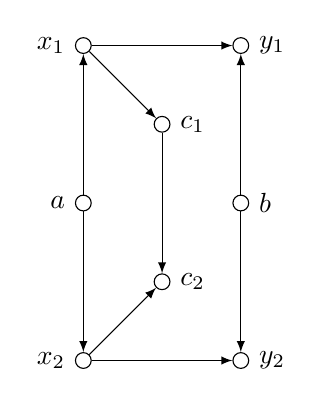
\begin{tikzpicture}
    [
    point/.style={circle,draw,inner sep=0pt,minimum size=2mm}
    ]
    \node (a) at (0,2) [point,label=left:$a$] {};
    \node (x1) at (0,4) [point,label=left:$x_1$] {};
    \node (x2) at (0,0) [point,label=left:$x_2$] {};
    \node (b) at (2,2) [point,label=right:$b$] {};
    \node (y1) at (2,4) [point,label=right:$y_1$] {};
    \node (y2) at (2,0) [point,label=right:$y_2$] {};
    \node (c1) at (1,3) [point,label=right:$c_1$] {};
    \node (c2) at (1,1) [point,label=right:$c_2$] {};
    \draw [-latex] (a) to (x1);
    \draw [-latex] (a) to (x2);
    \draw [-latex] (b) to (y1);
    \draw [-latex] (b) to (y2);
    \draw [-latex] (x1) to (y1);
    \draw [-latex] (x1) to (c1);
    \draw [-latex] (x2) to (y2);
    \draw [-latex] (x2) to (c2);
    \draw [-latex] (c1) to (c2);
  \end{tikzpicture}
  \caption{}
  \label{fig:open_door}
\end{figure}
As before, the vertices $y_1$, $y_2$ and $c_2$ are initial vertices of disjoint rays, and not sinks.

The NAND-clause we will show not to be binary-provable is $\ol{ab}$.
Figure~\ref{fig:v3_counter_proof} proves $\ol{ab}$, but the proof contains two non-binary NAND-clauses.
We will show that this is unavoidable.
\begin{figure}[!h]
  \centering
  \caption{}
  \label{fig:open_door_solution}
\end{figure}
\FloatBarrier
Based on these solutions, we can say a lot about the provability of various binary NAND-clauses.
Any pair of vertices from the graph that can be 1 under the same assignment will not be a Neg-provable NAND by soundness.
Also, since all the vertices can be assigned 1 under at least one assignment, no unary NAND can be proven in Neg.

We can make the following table showing what pairs of vertices can be 1 simultaneously and thus consititute a binary NAND unprovable in Neg.
A cell is filled with a reference to the assignment, if any, examplifying the case.
\[
\begin{array}{|c||c|c|c|c|c|c|c|c|}
  \hline
  & a & b & x_1 & x_2 & y_1 & y_2 & c_1 & c_2 \\ \hline\hline
  a & - & & & & \alpha_1 & \alpha_1 & \alpha_1 & \alpha_2 \\ \hline
  b & & - & \alpha_4 & \alpha_3 & & & \alpha_3 & \alpha_4 \\ \hline
  x_1 & & & - & & & \alpha_6 & & \alpha_6 \\ \hline
  x_2 & & & & - & \alpha_5 & & \alpha_5 & \\ \hline
  y_1 & & & & & - & \alpha_1 & \alpha_1 & \alpha_2 \\ \hline
  y_2 & & & & & & - & \alpha_1 & \alpha_2 \\ \hline
  c_1 & & & & & & & - & \\ \hline
  c_2 & & & & & & & & - \\ \hline
\end{array}
\]

Among the pairs above that are not shown to be unprovable, only two are not axioms: $\ol{ab}$ and $\ol{x_1x_2}$.
We will use this observation to show that it is impossible to prove $\ol{ab}$ with binary NAND-clauses only.

Let us assume that we have a rule application with all binary NAND-clauses in the premise and with $\ol{ab}$ in the conclusion.
Based on the (Rneg)-rule, we know that the premise must contain at least one binary NAND-clause containg $a$ and at least one containing $b$.
The table above tells us that the only provable binary NAND-clauses that contain $a$ or $b$ are the ones in the axiom set:
$\ol{ax_1}$, $\ol{ax_2}$, $\ol{by_1}$ and $\ol{by_2}$.
Since we don't want any $x_i$ or $y_i$ in the conclusion, these variables have to be removed by the OR-clause.
The OR-clauses $x_1y_1c_1$ and $x_2y_2c_2$ are the only ones that contain both an $x$ and a $y$, making them the only OR-clauses that can potentially conclude with $\ol{ab}$.

This gives us the following information: since both the possible OR-clauses are of length 3, the rule application concluding with $\ol{ab}$ has 3 NAND-clauses in its premise; one containing an $x$, one containing a $y$ and one containing a $c$.
Looking at our table again, we see that the potentially provable NAND-clauses containing a $c$ are again the axioms only.
Since there are no provable NAND-clauses on the form $ac_i$ or $bc_i$, we get that the conclusion of our rule cannot possibly be of length 2, thus contradicting our assumption.
We can therefore conclude that $\ol{ab}$ is \textit{not} binary-derivable, thus proving Theorem~\ref{thm:non_binary_derivable}.

\subsection{Inconsistencies}
\label{sub:Inconsistencies}
Consider now the following extension of our original graph:

\[
  \begin{tikzpicture}
    [
    point/.style={circle,draw,inner sep=0pt,minimum size=2mm},
    collection/.style={thick,rectangle,draw,inner sep=0pt,minimum height=14mm, minimum width= 9mm}
    ]
    \node (a) at (0,2) [point,label=left:$a$] {};
    \node (x1) at (0,4) [point,label=left:$x_1$] {};
    \node (x2) at (0,0) [point,label=left:$x_2$] {};
    \node (b) at (2,2) [point,label=right:$b$] {};
    \node (y1) at (2,4) [point,label=right:$y_1$] {};
    \node (y2) at (2,0) [point,label=right:$y_2$] {};
    \node (c1) at (1,3) [point,label=right:$c_1$] {};
    \node (c2) at (1,1) [point,label=right:$c_2$] {};
    \node (s) at (1,6) [point,label=left:$s$] {};
    \node (t) at (1,5) [point,label=below:$t$] {};
    \node (u1) at (-2,5) [point,label=left:$u_1$] {};
    \node (u2) at (4,5) [point,label=right:$u_2$] {};
    \draw [-latex] (a) to (x1);
    \draw [-latex] (a) to (x2);
    \draw [-latex] (b) to (y1);
    \draw [-latex] (b) to (y2);
    \draw [-latex] (x1) to (y1);
    \draw [-latex] (x1) to (c1);
    \draw [-latex] (x2) to (y2);
    \draw [-latex] (x2) to (c2);
    \draw [-latex] (c1) to (c2);
    \draw [-latex,loop right] (s) to (s);
    \draw [-latex] (s) to (t);
    \draw [-latex] (t) to (u1);
    \draw [-latex] (t) to (u2);
    \draw [-latex] (u1) to (a);
    \draw [-latex] (u2) to (b);
  \end{tikzpicture}
\]
The extension provides us with 6 new NAND-clauses and 4 new OR-clauses in the axioms set:
\begin{align}
  \text{OR'} &= \text{OR} \cup \{st,\; tu_1u_2,\; u_1a,\; u_2b \}\\
  \text{NAND'} &= \text{NAND} \cup \{\ol{s},\; \ol{st},\; \ol{tu_1},\; \ol{tu_2},\; \ol{u_1a},\; \ol{u_2b} \}
\end{align}

This extended graph can now be proven inconsistent using the newly provided clauses, as shown in the following Neg proof:
\begin{prooftree*}
  \Hypo{\ol{s}}
  \Hypo{\ol{tu_2}}
  \Hypo{\ol{tu_1}}
  \Hypo{\dots}
  \Infer1{\ol{ab}}
  \Infer[right label=$u_1a$]2{\ol{tb}}
  \Infer[right label=$u_2b$]2{\ol{t}}
  \Infer[right label=$st$]2{\varnothing}
\end{prooftree*}

We will now show that this inconsistency proof has to use the $\ol{ab}$ clause.

First of all, since both the vertices $s$ and $t$ are provably false, as the proof above shows, they can by soundness of Neg not be assigned 1 under any assignment.
This means that none of the binary NAND-clauses that contains either $s$ or $t$ can be ruled out as unprovable like we did above.

  % !TEX root= ../main.tex
\section{Unary NAND-clauses in graph theories}
\label{sec:Unary NAND-clauses in graph theories}
We will to use the fact that some binary NAND-clauses are not binary-derivable to show that some \textit{unary} NAND-clauses are not binary-derivable.

  \begin{tikzpicture}
    [
    ]
  \end{tikzpicture}

  \pagebreak % added to fix problem with floating of big graph
  \begin{lemma}
  Given the graph from Figure ... let the vertices $u$ and $v$ be from different components.
  If $\ol{uv}$ is binary-derivable, then its proof contains either $\ol{a^N}$, $\ol{a^W}$ or $\ol{a^E}$.
  \label{thm:uv_proof_contains_a}
\end{lemma}

\begin{proof}
  Base Case:
  No axiom $\ol{uv}$ exists such that $u$ and $v$ are vertices from different components, so our claim vacuously holds.

  Induction Step:
  Suppose we have a binary proof of $\ol{uv}$ where $u$ and $v$ are from different components.
  The immediate premise must contain at least one binary NAND-clause containing $u$ and one containing $v$.
  \begin{figure}[!h]
    \centering
    \begin{prooftree*}
      \Hypo{\ol{u\dots}}
      \Hypo{\ol{v\dots}}
      \Hypo{\dots}
      \Infer[]3{\ol{uv}}
    \end{prooftree*}
    \caption{}
    \label{fig:proof_scheme_uv}
  \end{figure}
  If either $u$ or $v$ are in a clause together with a vertex from a component different from their own, we get from the induction hypothesis that their proof must contain either $a^N$, $a^W$ or $a^E$, so we are done.

  Otherwise, $u$ and $v$ are each either in a clause together with the vertex $s$ or a vertex from their own component.
  Both of these cases results in using the OR-clause $sa^Na^Wa^E$ in the last proof step, since it is the only OR-clause containing $s$ and the only OR-clause containing vertices from different components.
  The premise therefore contains two additional NAND-clauses; one of them containing the $a$-vertex of the component not containing $u$ or $v$ - lets call it $a^w$.

  If the clause containing $a^w$ is unary, we are done.
  If the clause containing $a^w$ is binary, it must either contain $u$ or $v$ in order to give $\ol{uv}$ in the conclusion.
  Since $a^w$ is in a component different from both $u$ and $v$, the induction hypothesis gives us the claim.

  The proof must therefore contain either $a^N$, $a^W$ or $a^E$.
\end{proof}

\begin{lemma}
  $\ol{a^N}$, $\ol{a^W}$ and $\ol{a^E}$ are not binary-derivable.
  \label{thm:non_binary_derivable_a}
\end{lemma}

\begin{proof}
  We prove it by structural induction over the complexity of the proof tree.
  Base Case:
  Neither $\ol{a^N}$, $\ol{a^W}$ nor $\ol{a^E}$ are axioms, so the claim vacuously holds.

  Induction step:
  Suppose we have a binary proof of $\ol{a}$, where $a$ is either $a^N$, $a^W$ or $a^E$.
  Since the proof is binary, we get from our induction hypothesis that neither $\ol{a^N}$, $\ol{a^W}$ nor $\ol{a^E}$ appears in the proof.

  We get from Lemma~\ref{} that $\ol{a}$ is not binary-derivable using clauses from within its own component only, so the binary proof must use vertices outside the component containing $a$; either the $s$-vertex or vertices from other components.

  If it uses $s$, consider the last proof step with $s$ in the premise.
  The OR-clause used in this proof step must be $sa^Na^Wa^E$, being the only OR-clause containing $s$ and thus the only clause able to remove it.
  This OR-clause contains 4 vertices, so the premise must contain 3 additional NAND-clauses;
  one containing $a^N$, one containing $a^W$ and one containing $a^E$.
  We get the following restrictions on these 3 NAND-clauses.
  \begin{itemize}
    \item None of them can be unary, from the induction hypothesis.
    \item None of them can be binary and contain $s$, since that would give an $s$ in the conclusion, contradicting our assumption of this being the last proof step with $s$ in the premise.
    \item None of them can be binary and contain vertices from two different components, from the induction hypothesis and Lemma~\ref{thm:uv_proof_contains_a}.
  \end{itemize}
  The 3 additional NAND-clauses must therefore all contain a second vertex from their own component.
  Since the three component are disjoint, these three vertices are different, making the conclusion of the proof step non-binary, contradicting our original assumption of the proof being binary.

  If the proof does not contain $s$, then it uses some vertex $p$ from another component.
  Consider the last proof step with an ``external'' vertex in the premise.
  The proof step must remove $p$, and conclude with some clause containing vertices only from within the component containing $a$.
  The premise must obviously contain a NAND-clause containing $p$, but it must also contain at least one binary NAND-clause with a vertex from within N, in order to make the conclusion non-empty.
  That clause cannot contain any external vertices, from Lemma 1 and IH, so it must a clause with two N-vertices.
  The OR-clause used must therefore contain the external vertex $p$ and a vertex from N.
  $sa^Na^Wa^E$ is the only one with this property, but we have assumed that $s$ is not in this proof.

  $\ol{a}$ is thus not binary-derivable.

\end{proof}

\begin{corollary}
  $\ol{x^1x^2}$ is not binary-derivable.
  \label{thm:non_binary_derivable_uv}
\end{corollary}

\begin{proof}
  We get this directly from Lemma 1 and Lemma 2.
\end{proof}


  % !TEX root= ../main.tex
\section{Additional findings}
\label{sec:Additional findings}
While developing the proof of the refutational incompleteness of BNeg, some additional observations where made along the way.
Even though they ultimately didn't turn out useful for the main proof, they do bear some general significance.
These observations will be presented and proved in this section.

[TO BE WRITTEN]

  \chapter{Conclusion and future work}
  \label{chap:Conclusion and future work}
  % !TEX root= ../main.tex
This thesis has found various graph structures implying provability of certain NAND-clauses in Neg.
The process of continuously generalizing these structures has given several examples of unconventional graphs still providing certain provable clauses.
One of these exemplified that some provable binary NAND-clauses are not binary-derivable.
This example was further extended to show that Neg is \textit{not} refutationally complete when restricted to using binary NAND-clauses only.

In our context, this is primarily a negative result.
If BNeg \textit{was} refutationally complete, our search for a graph-structural equivalent of provable clauses would be easier, allowing us to assume that any clause is provable using binary NAND-clauses only.

Knowing this, one can move forward by trying to find other features of Neg.
One example is its non-explosiveness, mentioned in \cite{michal-completeness}
While classical proof systems are explosive and thus able to prove anything from inconsistent theories, Neg can only prove certain clauses.
It would be interesting to take a closer look at these clauses that are provable by the virtue of the graph being inconsistent, and potentially develop some definition of the ``explosive range'' of a graph.
Coming back to our original interest in paradoxes, this property becomes useful in attempts to identify and isolate the part of a theory that makes it paradoxical.
The concept of \textit{local kernels}, as defined and studied in \cite{synthese-pdl}, might contribute to this definition of an explosive range.

The non-explosiveness of Neg comes from the more general fact that Neg does not have \textit{weakening}, i.e. while rules like $\Gamma \vdash x \; \Rightarrow \; \Gamma \vdash x \vee y$ are admissible in classical proof systems, this is not the case for Neg.

Since Neg is not complete, it does not hold in general that $\Gamma \vDash \ol{A} \Rightarrow \Gamma \vdash \ol{A}$.
An interesting question might therefore be ``\textit{when} does it hold?''.
Corollary~5.1 from \cite{michal-completeness} tells us that $\Gamma \vDash \ol{A} \Leftrightarrow \exists B \subseteq A: \Gamma \vdash \ol{B}$.
A direct consequence of this is that $\Gamma \vDash \ol{A} \Rightarrow \Gamma \vdash \ol{A}$ holds when $\forall B \subset A: \Gamma \not\vdash B$ and by soundness also when $\forall B \subset A: \Gamma \not\vDash B$.
We can formalize this into a corollary on its own:
\begin{corollary}
  Given a graph $\mathbf{G} = \langle G,N \rangle$ and a set of vertices $A \subseteq G$, let $\Gamma = \mathcal{T}(\mathbf{G})$:
  \begin{align}
    \Gamma \vDash \ol{A} \wedge \forall B \subset A: \Gamma \not\vDash \ol{ B } \;\Rightarrow \; \Gamma \vdash \ol{A}
  \end{align}
\end{corollary}
In words, if no kernel in $G$ contains $A$, but for each subset $B \subset A$, there is a kernel that contains $B$, then $\ol{A}$ is provable in Neg.

Based on this observation, one might be able to find some interesting relations between the kernels in the graph and the set $A$.

Also, more work could be put into exploring graph structural relations $V$ such that for a graph and a subset $A$ of its vertices, we have $\Gamma \vdash \ol{A} \Rightarrow V(A)$.
The relation ``being connected in the underlying undirected graph'' is certainly such a relation, as shown in Section~\ref{sub:Isolated components}.
If one is able to strengthen that relation, it will probably make a bigger contribution to the proof of Walicki's conjecture than relations satisfying the inverse implication.

  \appendix
  \chapter{Proofs}
  \label{chap:Proofs}
  % !TEX root= ../main.tex
\section{Translating CNF to GNF}
\label{sec:Translating CNF to GNF}
Since any PL theory can be expressed in CNF, showing that any theory $P$ in CNF can be translated to a theory $R$ in GNF such that $P$ and $R$ are equisatisfiable gives us that any PL theory has an equisatisfiable GNF.

Given any CNF theory $P$, for each formula in it, follow the steps below to acquire its corresponding GNF theory.

\textbf{Step 1:}
For each atom $x_i$ in the formula, introduce a fresh variable $x'_i$ and add the following two GNF formulae to $P$:
$x'_i \lar \neg x_i, x_i \lar \neg x'_i,$ (unless this has already been done while translating an earlier formula in the theory).

\textbf{Step 2:}
In each clause of the formula, replace every negative literal $\neg x_i$ with its corresponding $x'_i$ fom step 1.
Every clause in the formula does now contain positive literals only.

\textbf{Step 3:}
For every clause $(x_1 \vee x_2 \vee \dots \vee x_n)$, replace it with the following formula, where $y$ is fresh:
\[y \lar (\neg x_1 \wedge \neg x_2 \wedge \dots \wedge \neg x_n \wedge \neg y)\]

This formula is equisatisfiable with our original clause.

The combined set of all these acquired formulae will make up our GNF-theory.
We have only added proper GNF formulae and all variables appear to the left in exactly one clause, so $R$ will indeed be a GNF theory.

Step 1 is adding a bi-implication formula that is always satisfiable, since one of two variables in it is fresh.
One can think of it as a labelling of an already existing variable.
Thus, adding these formulae to a theory does not change its satisfiability/non-satisfiability.

Step 2 is replacing each negative literal with its label, also not changing the satisfiability.

Step 3 is replacing one formula with an equisatisfiable formula, thus not changing the overall satisfiability.

Since none of the steps above change the satisfiability of the theory, we can conclude that our acquired theory is equisatisfiable with to original CNF theory.

Below are two examples of CNF-theories with their corresponding GNF-theories.\\
\begin{example}
  \begin{align}
    T1_{\text{CNF}}:\quad& ( a \vee b )\\
    T1_{\text{GNF}}:\quad& ( a \lar \neg a'), (a' \lar \neg a), (b \lar \neg b'), (b' \lar \neg b), (y_1 \lar (\neg a \wedge \neg b \wedge \neg y_1))\\
    T2_{\text{CNF}}:\quad& (\neg a)\\
    T2_{\text{GNF}}:\quad& ( a \lar \neg a'), (a' \lar \neg a), (y_1 \lar (\neg a' \wedge \neg y_1))
  \end{align}
\end{example}

	\pagebreak
	% !TEX root= ../main.tex
\subsection{Inconsistency of Stretched Yablo}
\label{sub:Inconsistency of Stretched Yablo}

One variation of the Yablo-graph is the Stretched Yablo-graph, presented by Walicki in \cite{michal-completeness}.
While the Yablo-graph is a ray where each vertex on it has direct edges to all the vertices after it, the Stretched Yablo-graph is a ray where each vertex has \textit{disjoint paths} (with certain properties depending on the variation of Stretched Yablo) to all vertices in after it.

The variation on which we will be proving an inconsistency is one with a set of core vertices $\mathbb{N}$ where each vertex $i$ has a disjoint path to every vertex $j$ after it, such that the length of the path is $(2 \times (j - i) - 1)$.

\begin{figure}[!h]
  \centering
  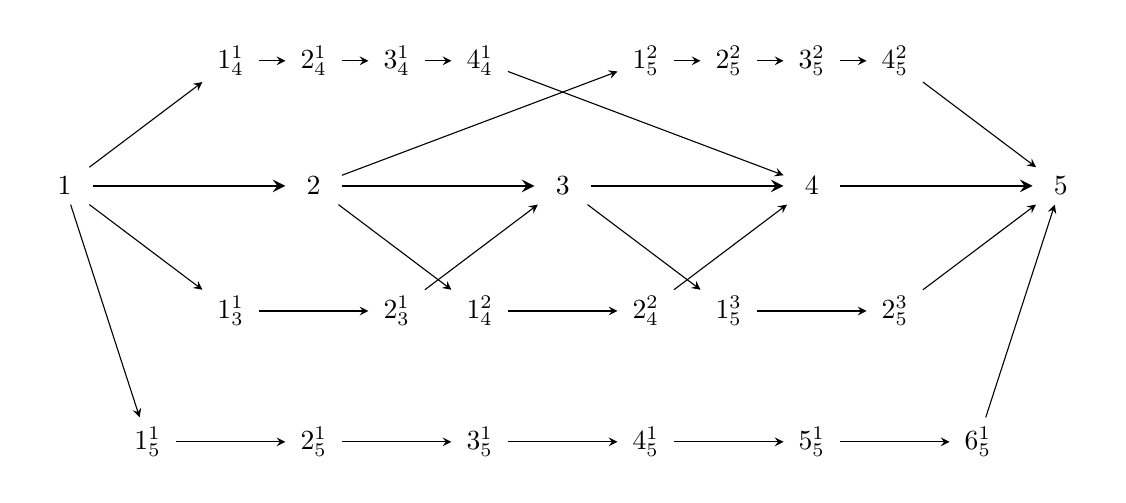
\begin{tikzpicture}
    [
    point/.style={circle,draw,inner sep=0pt,minimum size=2mm},
    collection/.style={thick,rectangle,draw,inner sep=0pt,minimum height=14mm, minimum width= 9mm}
    ]
	  \matrix (m) [matrix of math nodes,row sep=3em,column sep=1em,minimum width=2em]
	  {   & & 1^1_4 & 2^1_4 & 3^1_4 & 4^1_4 & & 1^2_5 & 2^2_5 & 3^2_5 & 4^2_5 & & \\
	  	1 & & & 2 & & & 3 & & & 4 & & & 5 \\
	  	  & & 1^1_3 & & 2^1_3 & 1^2_4 & & 2^2_4 & 1^3_5 & & 2^3_5 & & \\
		  & 1^1_5 & & 2^1_5 & & 3^1_5 & & 4^1_5 & & 5^1_5 & & 6^1_5 & \\
		};
	  \path[-stealth]
	  	(m-1-3) edge (m-1-4)
		(m-1-4) edge (m-1-5)
		(m-1-5) edge (m-1-6)
		(m-1-6) edge (m-2-10)
		(m-1-8) edge (m-1-9)
		(m-1-9) edge (m-1-10)
		(m-1-10) edge (m-1-11)
		(m-1-11) edge (m-2-13)
	  	(m-2-1) edge [line width=1pt] (m-2-4)
				edge (m-3-3)
				edge (m-1-3)
				edge (m-4-2)
		(m-2-4) edge [line width=1pt] (m-2-7)
				edge (m-3-6)
				edge (m-1-8)
		(m-2-7) edge [line width=1pt] (m-2-10)
				edge (m-3-9)
		(m-2-10) edge [line width=1pt] (m-2-13)
		(m-3-3) edge (m-3-5)
		(m-3-5) edge (m-2-7)
		(m-3-6) edge (m-3-8)
		(m-3-8) edge (m-2-10)
		(m-3-9) edge (m-3-11)
		(m-3-11) edge (m-2-13)
		(m-4-2) edge (m-4-4)
		(m-4-4) edge (m-4-6)
		(m-4-6) edge (m-4-8)
		(m-4-8) edge (m-4-10)
		(m-4-10) edge (m-4-12)
		(m-4-12) edge (m-2-13)
	  ;
	\end{tikzpicture}
  \caption{Stretched Yablo}
  \label{fig:stretched_yablo}
\end{figure}
Shown above are parts of the Stretched Yablo-graph described.
We denote the core vertices by natural numbers.
The peripheral vertices contained in each path is denoted by $n^x_y$ where $x$ and $y$ is the source and target, respectively, of the path in which the vertex is contained.
$n$ denoted the relative position on the path.

Using the above notation, we get the following sets of axioms from our graph:
\begin{align}
  N1a &= \{\; \ol{x(x+1)} \;&&|\; x \in \mathbb{N} \; \} \\
	N1b &= \{\; \ol{x1^x_y} \;&&|\; x,y \in \mathbb{N}, x+1 < y \; \} \\
	N2 &= \{\; \ol{n^x_y(n+1)^x_y} \;&&|\; n,x,y \in \mathbb{N}, x+1 < y, n < 2(y-x) - 2 \; \} \\
	N3 &= \{\; \ol{(2(y-x)-1)^x_yy} \;&&|\; n,x,y \in \mathbb{N}, x+1 < y \; \} \\
	O1 &= \{\; x(x+1)1^x_{x+2}1^x_{x+3}\dots \;&&|\; x \in \mathbb{N} \; \} \\
  O2 &= \{\; n^x_y(n+1)^x_y \;&&|\; n,x,y \in \mathbb{N}, x+1 < y, n < 2(y-x) - 2 \; \} \\
	O3 &= \{\; (2(y-x)-1)^x_yy \;&&|\; n,x,y \in \mathbb{N}, x+1 < y \; \}
\end{align}
We get that NAND = $N1a \cup N1b \cup N2 \cup N3$ and that OR = $O1 \cup O2 \cup O3$.
One can identify the different axioms by looking at the figure above\footnote{recall how NANDs corresponds to edges, while ORs corresponds to vertices}:
$N1a$ are the edges making up the core ray of the graph, $N1b$ are the edges going from a core vertex onto a peripheral vertex, $N2$ are the edges between two peripheral vertices and $N3$ are the edges going from a peripheral vertex back onto a core vertex.
$O1$ are the vertices on the core ray, $O2$ and $O3$ are the peripheral vertices, $O3$ being the ones that points back to a core vertex.

In order to prove $\varnothing$ from these axiom, we prove some intermediate clauses.

	\pagebreak
	% !TEX root= ../main.tex
\externaldocument{../binary_nands/odd_vels}
\section{Provability of NAND-clauses from vels}
\label{sec:Provability of NAND-clauses from vels}
This section will prove the following statement:
Given a graph where two vertices $a$ and $b$ are connected by a vel, as defined in Section~\ref{sec:Odd vels}, the binary NAND-clause $\ol{ab}$ is provable in Neg.

Let $\mathbf{G} = (G,N)$ be a graph containing the vertices $a,b$ such that they have a vel between them.
By definition, this means that there exists a vertex $c$ such that there is an oddly trimmed path from $a$ to $c$ and from $b$ to $c$, one of odd length and one of even length.

Let $P$ and $Q$ be the two sets containing the vertices in the path from $a$ to $c$ and from $b$ to $c$, respectively.
We will denote each element of $P$ as $p_i$ where $i \in \mathbb{N}$ is the position of that vertex in the path, starting at 0.
The elements of $Q$ will be named $q_i$ by the same rule.
We immediately have that $a = p_0$ and $b = q_0$.
As long as the trimming restrictions are met, $P$ and $Q$ might overlap, i.e. we might have cases where $p_j = q_k$ from some $i$ and $j$.

We assume, without any loss of generality, that the path from $a$ to $c$ is of odd length, making the path from $b$ to $c$.
We denote the lengths of the two paths by the numbers $n$ and $m$, giving us that $c = p_n = q_m$.
The path from $b$ to $c$ might also be empty, making $b = p_0 = c$.

This general variant of a vel can be illustrated in the following way, where the possibly branching vertices are shown with dashed edges out of them.
\begin{figure}[!h]
  \centering
  \begin{tikzpicture}
    [
    point/.style={circle,draw,inner sep=0pt,minimum size=2mm}
    ]
    \node (a) at (0,5) [point, label=left:${a = p_0}$] {};
    \node (p1) at (1,4) [point, label=left:$p_1$] {};
    \node (pd) at (2,3) [] {$\dots$};
    \node (pn2) at (3,2) [point, label=left:$p_{n-2}$] {};
    \node (pn1) at (4,1) [point, label=left:$p_{n-1}$] {};
    \node (c) at (5,0) [point, label=right:${c = p_n = q_m}$] {};
    \node (qm1) at (6,1) [point, label=right:$q_{m-1}$] {};
    \node (qm2) at (7,2) [point, label=right:$q_{m-2}$] {};
    \node (qd) at (8,3) [] {$\dots$};
    \node (q1) at (9,4) [point, label=right:$q_1$] {};
    \node (b) at (10,5) [point, label=right:${b = q_0}$] {};
    \draw [-latex] (a) to (p1);
    \draw [-latex] (p1) to (pd);
    \draw [-latex] (pd) to (pn2);
    \draw [-latex] (pn2) to (pn1);
    \draw [-latex] (pn1) to (c);
    \draw [-latex] (b) to (q1);
    \draw [-latex] (q1) to (qd);
    \draw [-latex] (qd) to (qm2);
    \draw [-latex] (qm2) to (qm1);
    \draw [-latex] (qm1) to (c);

    \node (e1) [below left=6mm and 4mm of c]  {};
    \node (e2) [below=8mm of c] {};
    \node (e3) [below right=6mm and 4mm of c] {};
    \draw [dashed] (e1) to (c);
    \draw [dashed] (e2) to (c);
    \draw [dashed] (e3) to (c);

    \node (ba) [below left=6mm and 4mm of a] {};
    \node (bn1) [below left=6mm and 4mm of pn1] {};
    \node (bb) [below right=6mm and 4mm of b] {};
    \node (bm2) [below right=6mm and 4mm of qm2] {};
    \draw [dashed] (ba) to (a);
    \draw [dashed] (bn1) to (pn1);
    \draw [dashed] (bb) to (b);
    \draw [dashed] (bm2) to (qm2);
  \end{tikzpicture}
  \caption{A general vel between $a$ and $b$}
  \label{fig:general_odd_vel}
\end{figure}

Let $\text{NAND}_G$ and $\text{OR}_G$ denote the axiomatic NAND- and OR-clauses we get from our graph.
We can work out the following subset of $\text{NAND}_G$:
\begin{align}
  \text{NAND}_V = \{\; \ol{p_ip_{i+1}} \;|\; 0 \leq i < n\;\} \;\cup\; \{\; \ol{q_jq_{j+1}} \;|\; 0 \leq j < m\;\}
\end{align}
Since both paths are oddly trimmed, every vertex at an odd position in its path will only have one out-edge, resulting in a binary OR-clause.
This makes us able to work out the following subset of $\text{NAND}_G$:
\begin{align}
  \text{OR}_V = \{\; p_ip_{i+1} \;|\; 0 \leq i < n, i\text{ is odd}\;\} \;\cup\; \{\; q_jq_{j+1} \;|\; 0 \leq j < m, j\text{ is odd}\;\}
\end{align}
The proof of $\ol{ab}$ can now be worked out, based only on the axioms $\Gamma_V = \text{NAND}_V \cup \text{OR}_V$:

\begin{figure}[h!]
  \begin{prooftree*}
    \Hypo{\ol{ap_1}}
    \Hypo{\ol{p_2p_3}}
    \Infer[left label=$p_1p_2$]2{\ol{ap_3}}
    \Hypo{\ol{p_4p_5}}
    \Infer[left label=$p_3p_4$]2{\ol{ap_5}}
    \Ellipsis{}{\ol{ap_{n-2}}}
    \Hypo{\ol{p_{n-1}c}}
    \Infer[left label=$p_{n-2}p_{n-1}$]2{\ol{ac}}
    \Hypo{\ol{bq_1}}
    \Hypo{\ol{q_2q_3}}
    \Infer[left label=$q_1q_2$]2{\ol{bq_3}}
    \Hypo{\ol{q_4q_5}}
    \Infer[left label=$q_3q_4$]2{\ol{bq_5}}
    \Ellipsis{}{\ol{bq_{m-3}}}
    \Hypo{\ol{q_{m-2}q_{m-1}}}
    \Infer[left label=$q_{m-3}q_{m-2}$]2{\ol{bq_{m-1}}}
    \Infer[left label=$q_{m-1}c$]2{\ol{ab}}
  \end{prooftree*}
  \caption{Proof that $a$ and $b$ are vel-connected}
  \label{fig:general_vel_proof}
\end{figure}

All the NAND-clauses used as axioms in the above proof are on the form $\ol{x_ix_{i+1}}$ and thus elements of $\text{NAND}_V$.
All the OR-clauses used as axioms are also on the form $x_ix_{i+1}$, and since $n$ is odd and $m$ is even, we see that all the OR-clauses used in the proof are indeed from $\text{OR}_V$.

Observe that the case where $b = c$ is unproblematic, since the above proof also proves $\ol{ac}$.
The case where some $p_i = q_j$ does not make any of the axioms change, making it too unproblematic.

All the axioms used are thus in $\Gamma_V$ which is a subset of $\Gamma_G$, and since all the rule applications are correct, our proof is valid.

  \pagebreak
  %% !TEX root= ../main.tex
\section{Axioms in Neg proofs}
\label{sec:Axioms in Neg proofs}
\begin{definition}
  A Neg proof is \textit{thin} if each rule application in the proof contains an axiomatic NAND-clause in its premise.
\end{definition}
In this section, we will prove the following statement:
\begin{theorem}
  Any NAND-clause provable in Neg has a thin proof.
\end{theorem}
Equivalently, for any Neg-proof $P$ there exists a thin Neg-proof with the same conclusion.
We will prove this theorem by inducing over the height of $P$.

  \chapter{Graph analysis}
  \label{chap:Graph analysis}
  % !TEX root= ../main.tex
\section{Provability of NAND-clauses in Figure~\ref{fig:double_open_door}}
\label{sec:Provability of NAND-clauses in double door}
Like the table in Figure~\ref{fig:v3_counter_table}, the following table shows what pairs of vertices from Figure~\ref{fig:double_open_door} can be 1 under the same solution and thus correspond to a binary NAND-clause unprovable in Neg.
\begin{figure}[!h]
  \centering
  \[\begin{array}{|c||c|c|c|c|c|c|c|c|c|c|c|c|c|c|c|c|c|c|}
    \hline
          & a & b^L & x^L_1 & x^L_2 & y^L_1 & y^L_2 & c^L_1 & c^L_2 & b^R & x^R_1 & x^R_2 & y^R_1 & y^R_2 & c^R_1 & c^R_2 & t\\ \hline\hline
    a     & & & & & & & & & & & & & & & & \\ \hline
    b^L   &-& X & X & X & & & X & X & X & X & X & X & X & X & X & \\ \hline
    x^L_1 &-&-& X & & & X & & X & X & X & X & X & X & X & X & \\ \hline
    x^L_2 &-&-&-& X & X & & X & & X & X & X & X & X & X & X & \\ \hline
    y^L_1 &-&-&-&-& X & X & X & X & X & X & X & & & X & X & \\ \hline
    y^L_2 &-&-&-&-&-& X & X & X & X & X & X & & & X & X & \\ \hline
    c^L_1 &-&-&-&-&-&-& X & & X & X & X & X & X & X & X & \\ \hline
    c^L_2 &-&-&-&-&-&-&-& X & X & X & X & X & X & X & X & \\ \hline
    b^R   &-&-&-&-&-&-&-&-& X & X & X & & & X & X & \\ \hline
    x^R_1 &-&-&-&-&-&-&-&-&-& X & & & X & & X & \\ \hline
    x^R_2 &-&-&-&-&-&-&-&-&-&-& X & X & & X & & \\ \hline
    y^R_1 &-&-&-&-&-&-&-&-&-&-&-& X & X & X & X & \\ \hline
    y^R_2 &-&-&-&-&-&-&-&-&-&-&-&-& X & X & X & \\ \hline
    c^R_1 &-&-&-&-&-&-&-&-&-&-&-&-&-& X & & \\ \hline
    c^R_2 &-&-&-&-&-&-&-&-&-&-&-&-&-&-& X & \\ \hline
    t     &-&-&-&-&-&-&-&-&-&-&-&-&-&-&-& \\ \hline
  \end{array}\]
  \caption{}
  \label{fig:double_door_counter_table}
\end{figure}

  \pagebreak
	\printbibliography
\end{document}
